%%%%%%%%%%%%%%%%%%%%%%%%%%%%%%
\documentclass[11pt]{report} 
\usepackage[a4paper, margin=2.5cm]{geometry} %set up margins 2.5cm
\usepackage{setspace}
\renewcommand{\baselinestretch}{1.5}  % increase line spacing
\usepackage{fontspec}
\setmainfont{Arial}
% MS Word style justification rather than latex-style hyphenation
\tolerance=1
\emergencystretch=\maxdimen
\hyphenpenalty=10000
\hbadness=10000
%%%%%% Figures 
\usepackage{graphicx} % for graphics
\usepackage{float} % to position graphics
\usepackage[labelfont=bf]{caption} 
\captionsetup[figure]{font={stretch=1.2}}    %% change 1.2 as you like
\usepackage[raggedright]{titlesec} %raggedright option = don't cut titles!
\usepackage{xcolor}
\definecolor{coolblack}{rgb}{0.0, 0.18, 0.39} %citations color
\usepackage[hyphens]{url}
\usepackage{hyperref}%for DOI
%\usepackage[url]
\hypersetup{colorlinks,linkcolor=black,urlcolor=teal,citecolor=teal} 
\setlength{\parindent}{0pt} % no paragraph indentation
\setlength{\parskip}{1em} %but a space
\usepackage{textcomp} % provides underscore
\usepackage{titletoc}% format TOC titles
\titlecontents{chapter}% <section-type>
  [0pt]% <left>
  {\bfseries}% <above-code>
  {\chaptername\ \thecontentslabel:\quad}% <numbered-entry-format>
  {}% <numberless-entry-format>
  {\hfill\contentspage}% <filler-page-format>
  
\usepackage{titlesec} % format chapters titles
\titleformat{\chapter}[display]
            {\normalfont\LARGE\bfseries}{\chaptertitlename\ \thechapter}{20pt}{\LARGE}[\vspace{2ex}\titlerule]
%per chapter numbering of tables and figures
\usepackage{chngcntr}
\counterwithin{figure}{chapter}
% mathematical equations
\usepackage{upgreek} % greek letters not in italic upalpha etc.
\usepackage{mathtools}
\numberwithin{equation}{section} % how the equation numbers are formed
\newtagform{show_eq}{(Eq.\ }{)}  % how the equation numbers are displayed
\usetagform{show_eq}
\usepackage{chngcntr} %Sequential equation numbering when using 'report' class
\counterwithout{equation}{chapter}
%bibliography:
\input{biblisettings.tex}
\bibliography{mybib280520.bib}
%%%%%%%%%%%%%%%%%%%%%%%%%%%%%%

\begin{document}

\begin{titlepage}
    \begin{center}
        Aus dem Juniorgruppe Ökologie und Evolution \\
        molekularer Parasit-Wirt-Interaktionen \\
        im Leibniz-Institut für Zoo- und Wildtierforschung \\
        des Fachbereichs Veterinärmedizin \\
        der Freien Universität Berlin
        
        \vfill
        \textbf{{\Large Resistance and tolerance to \textit{Eimeria} in the \\European house mouse hybrid zone}}
 
       \vfill
 
        Inaugural-Dissertation \\
        zur Erlangung des Grades eines \\
        PhD of Biomedical Sciences \\
        an der \\
        Freien Universität Berlin
 
        \vfill

        vorgelegt von \\
        Alice Christiane Anne-Marie Balard \\
        Tierärztin, MSc \\
        aus Rouen, Frankreich
        
        \vfill
        
        Berlin 2020 \\
        \textbf{Journal-Nr.: 4230}

    \end{center}
\end{titlepage}

\clearpage
\begin{center}
Gedruckt mit Genehmigung \\
des Fachbereichs Veterinärmedizin \\
der Freien Universität Berlin
\end{center}

\vspace{2cm}

\begin{tabular}{ l l l } 
\textbf{Dekan}: & Univ.- Prof. Dr. J\"urgen Zentek \\
\textbf{Erster Gutachter}: & Univ.-Prof. Dr. Heribert Hofer \\
\textbf{Zweiter Gutachter}: & Univ.-Prof. Dr. Emanuel Heitlinger \\
\textbf{Dritter Gutachter}: & Univ.-Prof. Dr. Justyna Wolinska \\
\end{tabular}

\vspace{2cm}

Deskriptoren (nach CAB-Thesaurus):\\
parasites, \textit{Eimeria}, \textit{Mus musculus}, hybridization, resistance, tolerance

\vspace{2cm}

Tag der Promotion: (noch nicht bekannt)

\clearpage

\pagenumbering{arabic} % start numbering from then on

\tableofcontents

\chapter*{List of abbreviations}
\addcontentsline{toc}{chapter}{List of abbreviations}
\begin{tabular}{l l}
Abbreviation & full term \\
\hline
AIC & Akaike information criterion \\
CI & confidence interval \\
Ct & cycle threshold \\
°C & degrees celsius \\
DNA & deoxyribonucleic acid \\
dpi & days post infection \\
F1 & first generation of crossing \\
F2 & second generation of crossing \\
F3 & third generation of crossing \\
F4 & fourth generation of crossing \\
Fig & figure \\
GTP & guanosine triphosphate \\
He & expected heterozygosity \\
HI & hybrid index \\
HMHZ   & European house mouse hybrid zone \\
IFNγ & interferon γ \\
km & kilometer \\
log2 & logarithm to the base 2 \\
MHC & major histocompatibility complex \\
min & minute \\
Mmd & \textit{Mus musculus domesticus} \\
Mmm    & \textit{Mus musculus musculus}  \\
mL & milliliter
\end{tabular}

\newpage

\begin{tabular}{l l}
Abbreviation & full term \\
\hline
NaCl & sodium chloride \\
OPG & oocysts per gram of feces \\
PCR & polymerase chain reaction \\
qPCR & quantitative polymerase chain reaction \\
s & second \\
sd & standard deviation \\
SIR & susceptible, infected, removed \\
Th1 & T helper type 1 \\
Th2 & T helper type 2 \\
ZINB &  zero-inflated negative binomial
\end{tabular}

\chapter{General introduction}
\section{Are parasites a selective force in the European house mouse hybrid zone?}
\subsection{Hybrids are not an average of their parents}
Species can be defined as groups of interbreeding natural populations that are reproductively isolated from each other (“biological species concept” proposed by \cite{mayr_animal_1963}). Hybrids appear when two species, or more largely two genetically distinct populations, meet and reproduce \citep{barton_analysis_1985}. Artificial animal hybridisation may be almost as old as selective animal breeding itself. The oldest known example is the mule, hybrid of a female horse and a male donkey, especially enduring, able to transport heavy burden, but sterile \citep{leighton_mule_1967}. 
\par
Hybrids can be superior than both parental populations for specific traits such as size, strength and growth. This phenomenon, called \textbf{heterosis} or \textbf{hybrid vigour}, is especially pronounced when parents come from two inbred populations \citep{brenner_heterosis_2001}. Hybrid vigour is maximum in the first generation of crossing, F1, where heterozygosity is at its highest. The \textbf{dominance hypothesis} states that the increase of heterozygosity in hybrids leads to the purge of deleterious recessive mutations in homozygous. According to the \textbf{overdominance hypothesis}, heterozygosity at one locus can even improve some traits compared to parents \citep{crow_overdominance_2001}. Overdominance is for example one of the possible explanations for the maintenance of high levels of genetic diversity of Major Histocompatibility Complex (MHC, set of genes coding for proteins involved in vertebrate immunity) \citep{read_major_2001, sommer_importance_2005}. Finally, interaction between genes could participate in hybrid vigour \parencite[\textbf{positive epistasis};][]{schnell_multiplicative_1992}, as was shown for the growth of the well-studied plant model, \textit{Arabidopsis thaliana} \citep{vanhaeren_combining_2014}.
\par
However, hybridisation does not necessarily result in hybrid superiority for all phenotypic traits. The heterozygous advantage can be counteracted by \textbf{genetic incompatibilities}. Firstly described by Bateson in the early 20th century \citep{bateson_heredity_1909}, these incompatibilities arise from the admixture of (at least) two alleles that have never before coexisted, and therefore create deleterious effects when brought together from distinct populations \citep{dobzhansky_studies_1936, muller_isolating_1942, orr_population_1995}. Later work on \textit{Drosophila} hybrids showed that these incompatibilities commonly involve three genes or more \citep{cabot_genetics_1994, palopoli_genetics_1994}, and interactions between genes \parencite[\textbf{negative epistasis};][]{larson_evolution_2018}. Hybrid incompatibilities can affect hybrid relative \textbf{fitness}, i.e. its reproductive success compared to other genotypes of the same population, in this case the parental genotypes \citep{krimbas_fitness_2001}. Total or partial \textbf{hybrid inviability} or \textbf{hybrid sterility} can act as reproductive barrier between two genetically distinct populations \citep{coyne_reproductive_2001}. In case of fertility decrease, Haldane first described that the heterogametic sex is the one more likely to be affected \citep{haldane_sex_1922}. Moreover, some \textbf{speciation genes} \parencite[genes underlying reproductive isolation;][]{wu_genes_2004} have been identified, mainly in \textit{Drosophila} genus \citep{oliver_accelerated_2009}. The \textit{prdm9} gene identified in mice is so far the only vertebrate gene known to participate in hybrid male sterility \citep{mihola_mouse_2009}. 
\par
Traditionally, hybrids were thought of as a rarity, but it seems now that a large proportion of plants (10\%) and animals (25\%) can produce hybrids in nature \citep{mallet_hybridization_2005}. Not only studying hybrids allows us to understand the mechanisms of speciation, but hybridisation with introduced species can threaten autochthonous endangered animals, making studies of hybridisation relevant for conservation biology \citep{simberloff_hybridization_1996}. \cite{stronen_perspectives_2013} also argue that the specific ecological role of hybrids could justify their protection by conservation policies. Moreover, hybrid zones represent melting pots of genotypes that allow to explore the impact of genetic diversity on several physiological systems (e.g. reproduction, immunity).
\par
In this thesis, we focus on a well studied system, the European house mouse hybrid zone (HMHZ).

\subsection{The European house mouse hybrid zone, a tension zone}
The house mouse (\textit{Mus musculus}) is the most widely used animal model in biomedicine. However, the vast majority of inbred lines used nowadays are not “natural” animals: they originate from pet mice from the late 19th and beginning of 20th century, and are mixtures of four different subspecies \citep{davisson_chapter_2004}. The common ancestor to all \textit{Mus musculus} subspecies originates from the Indo-Pakistani cradle. Several subspecies emerged after expansion from this cradle, commensal mice following human migrations \citep{boursot_evolution_1993}. At least five subspecies have been described based on phylogenetic analysis: \textit{M. m. musculus}, \textit{M. m. domesticus}, \textit{M. m. castaneus}, \textit{M. m. molossinus}, and \textit{M. m. gentilulus}. There is a wide range of evidence that these subspecies are not in complete reproductive isolation, and that gene flow can occur between them in zones of secondary contact \citep{auffray_house_2012}. In Europe, \textit{M. m. domesticus} (hereafter Mmd) and \textit{M. m. musculus} (hereafter Mmm) entered into secondary contact around the Bronze Age after having taken different colonisation routes, respectively south and north of the Black Sea, and, thus, diverging (mostly) in allopatry for about half a million years \citep{duvaux_isolation_2011, geraldes_inferring_2008, geraldes_higher_2011}. This secondary contact formed a belt of about 20 km wide and more than 2500 km long, running from Denmark to the Black Sea: the European house mouse hybrid zone (hereafter HMHZ) \citep{baird_what_2012, boursot_evolution_1993}(\textbf{Figure 1.1}). Despite the fact that they can form hybrids, these two subspecies differ in several traits including pelage color, tail/body length ratio (shorter for Mmm than for Mmd) \citep{boursot_evolution_1993}, boldness and activity \citep{frynta_behavioural_2018}, and male aggressiveness \citep{dureje_no_2010}.

\begin{figure}[H]
    \centering
    \includegraphics[width=.7\linewidth,height=\textheight,keepaspectratio]{images/1introduction/Figure1.pdf}
    \caption{Approximate course of the European house mouse hybrid zone (purple line) between \textit{Mus musculus domesticus} (blue) and \textit{Mus musculus musculus} (red) areas. (adapted from \cite{baird_where_2012}. Green square: Heitlinger group transect.}
\end{figure}

Through the HMHZ, the gene flow between both subspecies is not completely interrupted, and introgression of genes from one side to the other happens \citep{macholan_genetic_2007, macholan_assessing_2011, macholan_widespread_2019, raufaste_inferences_2005}. Hybrids between Mmd and Mmm are highly recombinant, presenting a range of genotypes, and no F1 or early-generation hybrids have been found \citep{macholan_genetic_2007}. Numerous genetic studies performed over geographically independent transects of the HMHZ \parencite[e.g.][]{macholan_genetic_2007, payseur_differential_2004, raufaste_inferences_2005} give strong support to the \textbf{tension zone} model in this system: the immigration of less hybridised mice to the centre of the zone, increasing the hybrid population size, is balanced by endogenous selection against hybrids \citep{baird_what_2012, barton_analysis_1985, boursot_evolution_1993}. This negative selection of hybrids seem to be linked with sterility or fertility \citep{baird_what_2012} and disruption of their spermatogenesis has been shown \citep{albrechtova_sperm-related_2012, martincova_sperm_2019, turner_reduced_2012, turner_genome-wide_2014}.
\par
Additionally, interaction with parasites (in this thesis, we will use the term “parasite” in the restricted eukaryotic sense, unless stated otherwise) has long been suggested to participate in the maintenance of the HMHZ. The next section will describe the long-lasting controversy around this issue.

\subsection{Parasites as hosts’ selective factor}
Parasites are ubiquitous in natural systems and affect human and animal health alike \citep{schurer_community-based_2016}. Their close interaction with their hosts over several generations and incentive to develop tactics to escape the host immune system led to consider parasites as plausible selective force for their hosts \citep{schmid-hempel_parasitesnew_2009}. There is evidence that parasites can manipulate vertebrate hosts behaviour, including the part related with reproduction \citep{klein_parasite_2003}. They can also affect their host community structure as was shown empirically in macroinvertebrates of New Zealand, where nematode density on cockles affect the full intertidal community \citep{mouritsen_parasites_2005}. It stands to reason that parasitic infections have been hypothesised to be a potential driving factor of maintenance or break-up of species barriers in hybrid zones \citep{sage_wormy_1986} (\textbf{Figure 1.2}).

\begin{figure}[H]
    \centering
     \includegraphics[width=.7\linewidth,height=\textheight,keepaspectratio]{images/1introduction/Figure2.pdf}
    \caption{\textbf{Hybrid fitness is reduced in the HMHZ} \citep{baird_what_2012}. Reproduction is negatively affected in hybrids, mainly via disruption of spermatogenesis (photography: various sperm heads from F1 experimentally produced hybrids. Figures A \& D: normal sperm heads; Figures B, C and E, F: abnormal sperm heads \parencite[source:][]{martincova_sperm_2019}. How hybrid health is affected by parasites is a long lasting debate.}
\end{figure}

The HMHZ is the first animal hybrid zone studied for differences in parasite loads \citep{sage_wormy_1986}. Original results seemed to indicate elevated worm load in hybrids. This was interpreted as hybrid incompatibilities: after having evolved separately within each subspecies, coadapted gene complexes in the immune system would be broken down in hybrids, which would lead to fitness reduction \citep{moulia_wormy_1991, moulia_experimental_1993, sage_wormy_1986}. However, further infection studies showed inconsistencies. Hybrids showed higher parasite loads compared to parents with the protozoan \textit{Sarcocystis muris} \citep{derothe_susceptibility_2001}, but reduced parasite loads (i.e. hybrid vigour on resistance) not only in F1 \citep{moulia_hybrid_1995} but also in later recombinant crossings F3 and F4 \citep{derothe_recombination_2004} following laboratory infection with helminths. More recently, a field study confirmed that hybrids had reduced helminth loads compared to parentals \citep{baird_where_2012}.
\par
All these different studies disagree on two major points: (1) the direction of hybrid effect of parasitism (are hybrids more resistant or more susceptible to parasites?) and (2) the role of parasites as selective factor. Indeed, to fully understand the possible impact of parasites on animals in the HMHZ, one must answer this question: does a change in parasite load necessarily imply a change in fitness? Before making assumptions on the impact of parasites on host fitness, there is a need to explore more thoroughly the different defense mechanisms of mice against parasites.

\section{Host immune defenses against parasites}
\subsection{Resistance and tolerance}

Parasites are by definition harmful to their hosts, and therefore imply costs \citep{noauthor_parasitism_2019}. These can be direct, including tissue damages and drain of host nutrients, or indirect, for instance, the decline of body condition that can lead to higher susceptibility to further infections \citep{beldomenico_poor_2008}, or by increasing susceptibility to predation \citep{bakker_parasite-induced_1997, ostlund-nilsson_parasitic_2005}. Hosts can defend themselves against parasitic infections in numerous ways. The first line of protection is provided by avoidance of parasites. If this strategy fails and the host gets infected, then the host immune system steps in \citep{schmid-hempel_evolutionary_2013}. \textbf{Resistance} is the ability of a host to reduce its pathogen burden. It results from host defense against infection or proliferation \citep{raaberg_decomposing_2009}. Resistance reduces parasite fitness by definition. However, when the immune response targeted at the parasite causes disease to the host (\textbf{immunopathology}), resistance can reduce host fitness too \citep{graham_evolutionary_2005}. 
\par
To deal with both the direct damages created by parasite infection and immunopathology, a second line of defense comes into play. \textbf{Disease tolerance} (not to be confused with immune tolerance which is the unresponsiveness of an immune system to a pathogen) is the ability of a host to reduce the damage induced by a certain parasite burden \citep{raaberg_decomposing_2009}, on health (\textbf{mortality tolerance}) or more indirectly on fecundity (\textbf{sterility tolerance}) \citep{best_maintenance_2008}. It is usually measured as the slope of a fitness trait, often a health measurement supposed to alter fitness eventually (e.g. body weight), on parasite load. It can be calculated in two ways: \textbf{range tolerance} measures a reaction norm, i.e. a change of phenotypic expression of the fitness trait in one genotype across a range of environments (in this case, several parasite loads). \textbf{Point tolerance} instead measures health at one single parasite load. These two measures can possibly give different results when different hosts present different health conditions when not infected with parasites, or when the relationship between health and parasite load is not linear \citep{little_coevolution_2010}. This can be problematic for field studies, where host health for a null parasite load and health-parasite load relationship are usually unknown, as confounding factors (e.g. coinfections, age, lactation status) come into play. Tolerance by definition increases the overall host fitness for a particular parasite load. Contrary to resistance, tolerance also increases parasite fitness, e.g. by providing parasite with a longer living niche, the host \citep{kutzer_maximising_2016, miller_evolution_2006, roy_evolutionary_2000}. 
\par
Resistance and tolerance are costly: in order to defend themselves against parasites, hosts consume resources that could have otherwise been used for other physiological functions \citep{sheldon_ecological_1996}. In the next section, we will examine the nature of the costs of defense mechanisms for the hosts. For the sake of conciseness, unless otherwise stated, we will focus on vertebrate hosts.

\subsection{Immune defenses are costly}
Resistance can result from a large range of mechanisms, from simple presence of unspecific biological barriers, to limitation of specific parasite growth. For the latter, the activation of innate and adaptive immune arms of the immune system comes with an energetic cost to the host \citep{schmid-hempel_evolutionary_2013}. This cost is typically measured by associating individual parasite load with fitness-associated functions. For example, resistance to parasites measured as (inverse of) fecal egg counts is reduced in lactating females in several animals including bighorn ewes \citep{festa-bianchet_individual_1989} and spotted hyena \citep{east_does_2015}. Lactation is a critical life-history stage for the survival of offspring and resource-demanding to the mother, hence it is hypothesised to be prioritised over maximum resistance to parasites.
\par
After establishment of infection, several mechanisms enter in action to increase tolerance, without targeting parasite growth, but rather the consequences of infection on host fitness. These mechanisms, much less studied than resistance mechanisms, mainly consist in protection from tissue damage or from alteration of host physiology, caused by pathogens or by the immune response \citep{medzhitov_disease_2012}. For example, \cite{reece_innate_2006} have showed that mice lungs inflammation induced by infection with the hookworm \textit{Nippostrongylus brasiliensis} is reduced by the induction of alternatively activated alveolar macrophages. In another rodent, field voles, \cite{jackson_immunological_2014} identified a mediator of Th2 immunity (the transcription factor Gata3) as tolerance marker, improving body condition and survival upon infection with macroparasites in mature animals. In this system, Gata3 was also negatively correlated with testis weight, suggesting a cost of tolerance in terms of reproductive effort.
\par
The optimal level of both defense mechanisms is determined by the balance between costs associated with parasitism, with resistance and with tolerance \citep{sheldon_ecological_1996}. Theory predicts that resistance alleles should present polymorphisms maintained by balancing selection, while tolerance alleles should evolve to fixation \citep{roy_evolutionary_2000, miller_evolution_2006}. Nevertheless, empirical studies do not all detect such pattern. Laboratory mouse strains infected with \textit{Plasmodium chabaudi} \citep{raaberg_disentangling_2007} present a negative correlation between resistance and tolerance (a given strain presenting intermediate levels of resistance and tolerance, high resistance and low tolerance, or vice versa). Similar results were found in infection of sea trout (\textit{Salmo trutta trutta}) and Atlantic salmon (\textit{Salmo salar}) with the trematode \textit{Diplostomum pseudospathaceum} \citep{klemme_vertebrate_2016}. This could be due to the redundancy of resistance and tolerance, resulting in trade-offs \citep{restif_concurrent_2004, fornoni_evolution_2004}. 
\par
\cite{kutzer_maximising_2016} noted that if studies addressing resistance are common, those addressing tolerance are more scarce. They suggest increasing the number of longitudinal studies and note that a host-centric view of tolerance is unsatisfactory, as host fitness also depends on the parasite \textbf{virulence}. In its strict sense, virulence means host mortality rate caused by parasite infection \citep{anderson_coevolution_1982}; in a more general sense evolutionary biologists sometimes use it as reduction of host fitness (health or fecundity) upon infection \citep{little_coevolution_2010}. For the reasons above developed, studying jointly resistance and tolerance is necessary to correctly assess the impact of parasites on their hosts. Importantly, this requires suitable host-parasite models, possibly with various levels of virulence in the same host.

\section{Our parasite model: \textit{Eimeria} spp.}
\subsection{\textit{Eimeria} spp. trigger a Th1 immune response}
We have seen earlier (1.3.) that the majority of studies (and all of the field studies) investigating the role of parasitism in the maintenance or break-down of species barrier in the European house mouse hybrid zone focused on helminths. As extracellular macroparasite, they trigger mainly a T helper type 2 (Th2) immune response \citep{sher_regulation_1992}. The effect of hybridization in terms of immune defenses of hybrid mice against parasites relatively to parental mice (higher, lower, or average) could depend on the type of immune response triggered. For this reason, we chose to focus our work on an intracellular microparasite genus, triggering a T helper type 1 (Th1)-mediated response \citep{sher_regulation_1992}, \textit{Eimeria}. In our second Chapter, we considered also helminths (more precisely pinworms) for comparison.
\par
The \textit{Eimeria} genus belongs to the phylum of Apicomplexan protozoan parasites. Their host range is extremely wide and includes birds, mammals, reptiles, amphibians and fish \citep{chapman_chapter_2013}. They are described particularly well in domestic animals due to their economical importance, especially in poultry \citep{blake_securing_2014}, but can also be found in wild animals, where they are potentially problematic for conservation \parencite{jeanes_two_2013, knowles_stability_2013, matsubayashi_molecular_2018}. Each of the >1800 described \textit{Eimeria} species is generally considered strictly host specific \citep{duszynski_eimeria_2011}, but the recent use of multilocus genetic markers method in rodents showed that this host specificity could be less strict than previously thought \citep{jarquin-diaz_generalist_2020}. \textit{Eimeria} oocysts, the infectious stage, are released in the environment via the feces and infect the next host by oral-fecal contamination. The parasites infect epithelial digestive cells of their hosts, which leads to malabsorption of nutrients and weight loss. The \textit{Eimeria} life cycle presents both asexual (schizogony) and sexual (gametogony) phases, and takes place in a single host \citep{burrell_life_2019}.
\par
\textit{E.~falciformis} is the gold standard for murine \textit{Eimeria} research. Host defense mechanisms against this parasite are well studied \parencite[see for example][]{mesfin_pathological_1978, pogonka_cd8_2010, schmid_apicomplexan_2012} and its whole genome is sequenced and annotated \citep{heitlinger_genome_2014}. T-cells have been shown to play a major role in the defense against \textit{E.~falciformis} infection \citep{mesfin_thymic_1979, stiff_effect_1990}. Following infection, interferon γ (IFNγ) is upregulated \citep{schmid_eimeria_2014}, and experimental infections showed higher weight loss and pathology but lower oocysts shedding in IFNγ-deficient mice than in wild type \citep{stange_il-22_2012}. IFNγ could in this respect be seen as a tolerance factor. \cite{ehret_dual_2017} compared host and \textit{E.~falciformis} transcriptomes (dual transcriptomes) in immunocompetent and immunodeficient laboratory mice, and in naïve and challenged laboratory mice. They did not find differences in the gene expression profile of this parasite between hosts, and concluded that \textit{E.~falciformis} does not respond plastically to the host environment but rather present a genetically canalised (“hard wired”) program of infection. 
\par
By considering \textit{Eimeria} spp. and helminths jointly, triggering Th1 and Th2 immune responses, we attempted to assess the generality of hybrid response in nature (\textbf{Chapter 1}). On a note of caution, in the field, one can only assess the impact of parasite species that are prevalent enough to allow robustness of statistical tests. Using a complementary laboratory approach can solve this issue (\textbf{Chapter 2}).
\subsection{Focus on two \textit{Eimeria} species: \textit{E.~falciformis} and \textit{E.~ferrisi}}
In a recent study performed by our group in the HMHZ, three \textit{Eimeria} species have been identified: \textit{E.~ferrisi}, \textit{E.~falciformis}, and \textit{E. vermiformis} with prevalences of 16.7\%, 4.2\% and 1.9\%, respectively \citep{jarquin-diaz_detection_2019}. Current markers were not able to detect a population structure for \textit{Eimeria} spp. in the HMHZ \citep{jarquin-diaz_generalist_2020}. The two most prevalent \textit{Eimeria} species, \textit{E.~ferrisi} and \textit{E.~falciformis}, present close ecological niches \parencite[\textit{E.~ferrisi} infects the cecum villar epithelial cells and \textit{E.~falciformis} the cecum crypt cells;][]{schito_comparison_1996}, but different virulence in laboratory mice. More precisely, the life cycle of \textit{E.~ferrisi} is shorter than that of \textit{E.~falciformis} \citep{al-khlifeh_eimeria_2019, schito_comparison_1996}. They both provoke similar symptoms in laboratory mice, mainly diarrhea, lesion of the enteric epithelium, and weight loss \citep{ankrom_life_1975, ehret_dual_2017, schito_comparison_1996}. In a study using the laboratory Swiss mouse strain, \cite{tilahun_oocyst_1981} found a higher mortality rate for \textit{E.~ferrisi} (2 out of 5 mice died when infected with 10$^5$  oocysts) than for \textit{E.~falciformis} (no death observed for the same inoculum). Though, they note that a former study described another isolate of \textit{E.~falciformis} far more lethal, killing mice from an inoculum of 2000 oocysts \citep{mesfin_pathological_1978}. More recently, using a lower infective dose (200 oocysts) on the laboratory NMRI mouse strain, we observed a stronger virulence of two different isolates of \textit{E.~falciformis} compared with one of \textit{E.~ferrisi}, both in terms of weight loss and mortality, correlated with a stronger immunopathology \citep{al-khlifeh_eimeria_2019}. The observed discrepancies in these in vivo experiments can be due to potential attenuation of virulence in case oocysts are collected early in the infection cycle \citep{mcdonald_endogenous_1987}, to modified virulence of specific parasite isolate over time in the lab, or to different immune systems of each mouse strain. \textit{E.~ferrisi} has been less intensively studied than \textit{E.~falciformis}; nevertheless, mortality after infection and oocysts output were found to differ between eight tested laboratory mouse strains, and T-cells also play a role in resistance to this parasite \citep{klesius_strain-dependent_1979}.
\subsection{Proxies for resistance and tolerance to \textit{Eimeria} spp.}
Resistance against murine \textit{Eimeria} species can be estimated by the inverse of parasite load. In our field study (\textbf{Chapter 2}), \textit{Eimeria} load was measured by the quantity of parasite gene in the infected tissues (ileum and caecum) per mouse gene. We also assessed the impact of infection on host health: body condition was calculated as individual residuals from ordinary least-squares regression of body weight by body length (separately for males and females). of note, this is not an estimation of tolerance, as individual weight before infection cannot be known in the field (apart from capture-marked-recapture, an approach that we excluded as it would have significantly reduced the number of mice and locations visited). 
\par
Our complementary laboratory experiment (\textbf{Chapter 3}) allowed us to measure the parasite load (oocysts count per gram of feces) in the same individual along the course of infection. We found it correlated with parasite load at the peak of infection, and used this second measurement as a proxy for (inverse of) resistance. More importantly, tolerance could be estimated for each mouse genotype, as a reaction norm, i.e. a relative weight loss across a range of parasite load. 
\section{Aims of this thesis}
\textbf{Aim 1. Investigating the effect of host hybridisation on resistance to parasites in the HMHZ}. Previous studies lead to conflicting results, hybrid mice being found either more resistant to parasites than parental subspecies, or less resistant. To solve this disagreement and address the generality of hybrid response, we considered simultaneously our protozoan model (\textit{Eimeria} spp.) and helminths (pinworms). We did so in a new transect of the HMHZ, including four years of mice sampling. To distinguish between interpretations of parasitemia we asked if (i) parasite loads are higher or lower in hybrids compared to parentals, and (ii) if these loads are consistent, or differ, between prevalent representative helminth and protozoan species. This topic is covered in Chapter 2.
\par
\textbf{Aim 2. Testing the coupling of resistance and tolerance against two murine \textit{Eimeria} species}. These two defense mechanisms could be positively correlated, traded-off against each other, or decoupled, the level of one defense mechanism not affecting the other. Conclusions on tolerance to parasites, and ultimately fitness, cannot be drawn without an understanding of this potential coupling. In a laboratory infection, we asked if \textit{E.~ferrisi} and \textit{E.~falciformis} showed the same resistance and tolerance patterns in both Western (Mmd) and Eastern (Mmm) hosts. This topic is covered in Chapter 3. 

 
\chapter{Intensity of infection with intracellular \textit{Eimeria spp.} and pinworms is reduced in hybrid mice compared to parental subspecies}
(Published article) \par

Alice Balard, V{\'{\i}}ctor Hugo Jarqu{\'{\i}}n-D{\'{\i}}az, Jenny Jost, Iva Martincov{\'{a}}, {\v{L}}udov{\'{\i}}t {\v{D}}ureje, Jaroslav Pi{\'{a}}lek, Milo{\v{s}} Machol{\'{a}}n, Joëlle Go\"{u}y de Bellocq, Stuart J. E. Baird and Emanuel Heitlinger \par
  
\textit{Journal of Evolutionary Biology} (2020), 33(4), 435–448 \\
doi: \url{https://doi.org/10.1111/jeb.13578}\\

\textbf{Author contibutions:}\\
All authors contributed to the conception and design of the analysis. A.B., V.H.J.D, J.J., I.M., L.D., M.M. and E.H. contributed to the data collection. A.B led the data analysis with the support of all authors. A.B. and E.H. led the writing of the manuscript, and all other authors provided editorial advice. \par

\newpage

\section{Abstract}
Genetic diversity in animal immune systems is usually beneficial. In hybrid recombinants, this is less clear, as the immune system could also be impacted by genetic conflicts. In the European house mouse hybrid zone, the longstanding impression that hybrid mice are more highly parasitized and less fit than parentals persists despite the findings of recent studies. Working across a novel transect we assessed infections by intracellular protozoans, \textit{Eimeria} spp., and infections by extracellular macroparasites, pinworms. For \textit{Eimeria} we found lower intensities in hybrid hosts than in parental mice but no evidence of lowered probability of infection or increased mortality in the centre of the hybrid zone. This means ecological factors are very unlikely to be responsible for the reduced load of infected hybrids. Focusing on parasite intensity (load in infected hosts) we also corroborated reduced pinworm loads reported for hybrid mice in previous studies. We conclude that intensity of diverse parasites, including the previously unstudied \textit{Eimeria}, is reduced in hybrid mice compared to parental subspecies. We suggest caution in extrapolating this to differences in hybrid host fitness in the absence of, for example, evidence for a link between parasitemia and health.

\textbf{Keywords: parasites, hybridization, resistance}

\section{Introduction}
The relevance of hybridization, producing individuals admixed between genetically distinct populations, is increasingly recognized by biologists. \cite{mallet_hybridization_2005} suggested that hybridization occurs in more than 10\% of animal species and 25\% of vascular plant species. Recently, the realization that humans are also a product of hybridization has raised interest further \citep{green_draft_2010}. In a conservation context hybridization with introduced species can threaten autochthonous endangered animals \citep{simberloff_hybridization_1996}. Parasites are omnipresent in natural systems and impact human and animal health \citep{schurer_community-based_2016}. It is therefore important for biologists to comprehend the interplay between parasites and hosts under hybridization.
\par The European house mouse hybrid zone (HMHZ), one of the first animal hybrid zones studied for differences in parasite loads \citep{sage_wormy_1986}, is a tension zone characterized by selection against hybrids replaced by immigrating less admixed mice \citep{barton_analysis_1985}. After ~500 000 years of (mostly) allopatric divergence two house mouse subspecies, \textit{Mus musculus domesticus} and \textit{Mus musculus musculus} (hereafter Mmd and Mmm), have come into secondary contact in Europe as a result of different colonization routes south and north of the Black Sea, respectively \citep{boursot_evolution_1993, duvaux_isolation_2011}. The HMHZ is about 20 km wide and more than 2500 km long, running from Scandinavia to the coast of the Black Sea \citep{baird_what_2012, boursot_evolution_1993, jones_norwegian_2010, macholan_location_2003}. This zone represents a semi-permeable barrier to gene flow between the two taxa \citep{macholan_genetic_2007, macholan_assessing_2011}. The main selective forces acting against hybrids are thought to be endogenous rather than ecological \citep{baird_what_2012, boursot_evolution_1993}, for example disruption of spermatogenesis in hybrids \citep{albrechtova_sperm-related_2012, turner_reduced_2012}.
\par Hybrids in tension zones have reduced fitness compared to individuals with “parental” genotypes due to genetic incompatibilities revealed on parentals’ secondary contact \citep{barton_analysis_1985}. As different components of fitness can vary independently, the immune system of hybrids might either benefit from recombinant genetic heterogeneity or suffer from incompatibilities. In the case of benefit we might expect decreased parasite load in hybrid individuals; in the case of incompatibilities we might expect increased load in hybrid individuals, compared to parental hosts. Parasites are traditionally seen as decreasing their hosts’ fitness, and differences in resistance to parasites between hybrid and pure hosts were suggested to affect the dynamics of hybrid zones \citep{fritz_resistance_1999}. An involvement of parasites in the maintenance or breakdown of species barriers, however, has never been clearly justified or demonstrated \citep{baird_shifting_2019}. In the HMHZ system, there is disagreement on both the direction of effects of hybridization on parasites \parencites[see][vs]{sage_wormy_1986, moulia_wormy_1991}{baird_where_2012} and on the interpretation of these findings with regards to host fitness and hybridization \parencites[see for example][]{theodosopoulos_parasites_2019, baird_shifting_2019}.
\par Initial results on parasites obtained in the HMHZ and experimental studies seemed to indicate elevated parasite loads in hybrids. This has been interpreted as potentially leading to fitness reductions in hybrids, hampering hybridization and thus reinforcing species barriers \citep{moulia_wormy_1991, moulia_experimental_1993, sage_wormy_1986}. Infection experiments using the protozoan Sarcocystis muris led to a similar conclusion \citep{derothe_susceptibility_2001}. Other laboratory experiments, however, showed either no effect in inter-subspecies F1s on helminth load or even reduced load in inter-subspecies F1s compared to pure mouse strains \citep{derothe_recombination_2004, moulia_hybrid_1995}. In 2012, more than two decades after the original field studies \citep{moulia_wormy_1991, sage_wormy_1986}, Baird et al. found, (with much larger sample size, clearer sampling design and more up to date inference), reduced helminth loads in hybrid mice \citep{baird_where_2012}, especially for the pinworms \textit{Aspiculuris tetraptera} and \textit{Syphacia obvelata} and the whipworm \textit{Trichuris muris}. It should be noted that the design of the field studies preceding the \cite{baird_where_2012} reappraisal usually suffered from low sample sizes and/or maintenance of mice under laboratory conditions before assessment of parasite burden, which may have allowed spurious signal to dominate the results. Nevertheless, even the basic direction of parasite load differences in hybrid mice compared to parental genotypes still seems controversial to some researchers. 
\par We now see that, despite working within the framework of the same hybrid zone, two different interpretations of parasite loads in hybrid mice have arisen. It should be noted that all the previous studies chose to focus on either helminth or protozoan parasite models. In vertebrates, the immune mechanisms of parasite control differs greatly between these two groups. Extracellular macroparasites like helminths trigger a T helper type 2 (Th2) -dominated response, and intracellular microparasites like protozoa trigger a T helper type 1 (Th1) -mediated response \citep{sher_regulation_1992}. One way forward in such circumstances is to test hypotheses over replicates and “along different axes” of parasitism, and to consider simultaneously helminths and protozoans to address the generality of hybrid response. To distinguish between interpretations of parasite load we here asked if (1) parasite loads are higher or lower in hybrids compared to parentals, and (2) if these loads are consistent, or differ, between prevalent representative helminths and protozoa. We did so in a geographically new transect replicate of the HMHZ.
\par Pinworms (oxyurids) have been detected in mice in numerous field studies \parencites[see for example][]{behnke_aspiculuris_1975, behnke_aspiculuris_1976,kriska_parasitic_1993, ressouche_host_1998}. They have been shown to be the most prevalent helminths infecting house mice in the HMHZ \citep{gouy_de_bellocq_new_2012}. They are often considered to provoke mild symptoms on their hosts, even if in rare conditions (e.g. particularly high burden) they have been shown to affect the health of laboratory mice \citep{taffs_pinworm_2016}. \textit{Eimeria} spp. are often considered host-specific, with several thousand species parasitizing different vertebrates \citep{chapman_chapter_2013, haberkorn_entwicklung_1970}. These parasites infect the intestinal epithelial cells of vertebrates and induce symptoms such as weight loss and diarrhoea. For example, infecting the NMRI mouse laboratory strain with \textit{Eimeria} oocysts isolated from mice captured in the HMHZ resulted in a weight loss up to 20\% compared to control \citep{al-khlifeh_eimeria_2019}. In the European HMHZ, three \textit{Eimeria} species have been identified: \textit{E.~ferrisi} , \textit{E.~falciformis} , and \textit{E. vermiformis}  with prevalences of 16.1\%, 4.2\% and 1.1\%, respectively \citep{jarquin-diaz_detection_2019}. 
\par We assessed \textit{Eimeria} infection in a novel transect of the HMHZ in Brandenburg, northeastern Germany, in which the hypothesis of hybrid resistance/susceptibility to parasite had never before been tested. We assessed the impact of host hybridization on intensity of this parasite. By focusing on parasite intensity \parencite[extent of parasite infection in only infected animals;][]{bush_parasitology_1997}, we arguably exclude ecological factors for differences in load. We show that (1) parasite loads are consistently lower in hybrids compared to parental genotypes in the HMHZ and (2) that this pattern is similar for our intracellular and extracellular parasite models.

\section{Material \&  Methods}
\subsection{Sampling}
Our sampled individuals consist of 660 house mice trapped using live traps placed in farms or houses between 2014 and 2017. The study area ranges from 51.68 to 53.29 degrees of latitude (200 km) and from 12.52 to 14.32 degrees of longitude (140 km). Each year mice were trapped in September when it is possible to capture a high number of mice in this region. In addition, sampling at the same season every year reduces potential seasonal variation \citep{abu-madi_seasonal_2000, haukisalmi_population_1988}. The locations for trapping were selected across a geographical range allowing both parental and hybrid/recombinant individuals to be captured. Mice were individually isolated in cages and then euthanized by isoflurane inhalation followed by cervical dislocation within 24 hours after capture (animal experiment permit No. 2347/35/2014). Individual mice were measured (body length from nose to anus), weighted, and dissected. Tissue samples (muscle and spleen) were transported in liquid nitrogen and stored at -80°C for subsequent host genotyping. Digestive tracts were dissected and inspected for helminth parasites (see below). Ileum, caecum and colon tissues were frozen in liquid nitrogen and then stored separately at -80°C. A median of 2 mice per locality were captured. A table of individual mouse data including hybrid indices, georeferences and parasite loads is available in \textbf{Supplementary Table S2.3}. To investigate \textit{Eimeria} infections we checked 384 mice sampled in 2016 and 2017 for the presence and intensity of tissue stages (\textbf{Figure~2.2a}). Between 2014 and 2017, 585 mice were investigated for helminths (\textbf{Figure~2.3a}). 

\subsection{Host genotyping}
The admixture of mouse genomes across the HMHZ was estimated for each mouse as a value of the hybrid index (HI) calculated as a proportion of Mmm alleles in a set of 14 diagnostic markers. This set consists of one mitochondrial marker \parencite[BamHI, a restriction site in the Nd1 gene;][]{bozikova_mitochondrial_2005, munclinger_genetic_2002} one Y-linked marker \parencite[presence/absence of a short insertion in the Zfy2 gene;][]{boissinot_discordant_1997, nagamine_musculus-type_1992}, six X-linked markers (three B1 and B2 short interspersed nuclear elements in Btk, Tsx \citep{munclinger_b1_2003}, and Syap1 \citep{macholan_genetic_2007}, X332, X347 and X65 \citep{dufkova_inference_2011, dureje_mouse_2012}), and six autosomal markers \parencite[Es1, H6pd, Idh1, Mpi, Np, Sod1;][]{macholan_genetic_2007}. HIs ranged from 0 to 1, HI of 0 indicating a pure Mmd and HI of 1 a pure Mmm \citep{baird_what_2012, macholan_genetic_2007}. At least 10 loci provided information for 92\% of the mice, and at least 4 loci for the remaining 8\% due to technical issues. Histograms for the number of genotyped markers, as well as their distribution across the hybrid index indicate no bias in genotyping (\textbf{Supplementary Figure S2.1}). 
\par The expected centre of the HMHZ across the study area was estimated using the program Geneland v4.0.8 (with graphical resolution increased over defaults, the modified code is available at \url{https://github.com/alicebalard/Geneland} as a complete R-package), based on a subset of the six autosomal markers that were genotyped in all individuals with 6 diploid markers (N=598 mice). Geneland uses a Markov chain Monte Carlo (MCMC) approach to combine both geographical and genetic information \citep{guillot_geneland_2005}. The number of clusters was set to 2, 106 MCMC iterations were performed and saved every 100th iterations (104 iterations saved). The first 200 iterations were discarded as burn-in and the resolution of the map was set to 2000 pixels for the x axis and 1400 for the y axes corresponding roughly to 1 pixel for 100m \citep{macholan_assessing_2011}.

\subsection{Parasite load estimation}
Mouse digestive tracts were dissected and inspected for helminth presence with a binocular microscope. Helminths were counted and stored in 70\% ethanol for later identification by molecular analysis and, when more than one worm per host was present, in 3.5\% formalin for later morphological comparison with species descriptions. As in this study we required high statistical power to test our hypotheses, we considered only the most prevalent helminths, the oxyurids \textit{Syphacia obvelata} and \textit{Aspiculuris tetraptera}. Histograms presenting the distribution of  counts for other helminths can be found in \textbf{Supplementary Figure S2.2} and data is available in \textbf{Supplementary Table S2.3}.

\par 
DNA was extracted from ileum and caecum tissues and quantitative PCR (qPCR) was used for estimation of \textit{Eimeria} spp. load. DNA extraction was performed using the innuPREP DNA Mini Kit (Analytik Jena AG, Jena, Germany) following the instructions of the manufacturer with additional mechanical tissue disruption with liquid nitrogen in a mortar. Both quality and quantity of isolated DNA were measured by spectrophotometry in a NanoDrop 2000c (Thermo Scientific, Waltham, USA). The presence of \textit{Eimeria} spp. was tested using qPCR to detect intracellular stages of the parasite as well as a house mouse house-keeping gene as internal reference. Primers used for \textit{Eimeria} spp. detection targeted a short mitochondrial COI region (Eim\textunderscore COI\textunderscore qX-F:  TGTCTATTCACTTGGGCTATTGT; Eim\textunderscore COI\textunderscore qX-R: GGATCACCGTTAAATGAGGCA), while \textit{Mus musculus} primers targeted the CDC42 nuclear gene \parencite[Ms\textunderscore gDNA\textunderscore CDC42\textunderscore F: CTCTCCTCCCCTCTGTCTTG; Ms\textunderscore gDNA\textunderscore CDC42\textunderscore R: TCCTTTTGGGTTGAGTTTCC; ][]{al-khlifeh_eimeria_2019, jarquin-diaz_detection_2019}.
\par These qPCRs have been independently confirmed with respect to detection of experimental infection \citep{al-khlifeh_eimeria_2019} and with genotyping PCRs using different primers and markers \citep{jarquin-diaz_detection_2019}. Reactions were performed using 1X iTaqTM Universal SYBR® Green Supermix (Bio-Rad Laboratories GmbH, München, Germany), 400 nM of each primer and 50 ng of DNA template in 20 µL final volume. Cycling amplification was carried out in a Mastercycler® RealPlex 2 thermocycler (Eppendorf, Hamburg, Germany) with the following amplification program: 95°C initial denaturation (2 min) followed by 40 cycles of 95°C denaturation (15 s), 55°C annealing (15 s) and 68°C extension (20 s). Melting curve analyses were performed in order to detect primer dimer formation and unspecific amplification. ΔCt was calculated as difference of the threshold cycle (Ct) between mouse and \textit{Eimeria} spp. values (corresponding to a log2 ratio between parasite and mouse DNA). This method was validated in an infection experiment of NMRI mice \citep{al-khlifeh_eimeria_2019}. We considered ΔCt=-5 our limit of detection as at this limit it was possible to obtain genotyping data for all samples using independent PCR reactions \citep{ahmed_novel_2019, jarquin-diaz_detection_2019}. Samples with a ΔCt lower than -5 were considered negative (unspecific signal due to amplification of non-target DNA). Samples with a ΔCt higher than -5 for at least one of the two intestinal tissues were considered positive, and in the case of detection in both tissues, the higher value was taken as a proxy of individual parasite load. This parasite load of the intestinal tissue stage is denoted as “ΔCtMouse−\textit{Eimeria}” throughout the following. \textit{Eimeria} identification at the species level was performed by means of two PCR markers (18S and COI) followed by a confirmation of morphology and tissue preference as described in \cite{jarquin-diaz_detection_2019} (column “eimeriaSpecies” of \textbf{Supplementary Table S2.3}).

\subsection{General parasite assessment}
As the distributions of parasite loads are expected to be highly skewed \citep{bliss_fitting_1953}, the median (as an estimator for the mode) is more informative than the mean \citep{rozsa_quantifying_2000}. We therefore report the median of parasite load across all hosts (median abundance) and of parasite load of infected host (median intensity) for pinworms, and only median intensity for \textit{Eimeria} spp. For qPCR some uninfected samples present technical noise due to unspecific amplification of non-target DNA. We therefore used a qPCR threshold validated by independent genotyping PCRs \parencite[see “Fig. 4” of][]{jarquin-diaz_detection_2019} to establish the infection status of each sample \parencite[and we do not report abundance for \textit{Eimeria}, see][for details]{jarquin-diaz_detection_2019}. Prevalence (relative frequency of infected individuals amongst all tested individuals) confidence intervals were obtained with Sterne’s exact method \citep{reiczigel_exact_2010, sterne_remarks_1954}. Calculations were performed using the epiR package \citep{nunes_epir_2018} running within the R statistical computing environment \citep{R_2010}.

\subsection{Statistical design: testing hybrid resistance/susceptibility in a natural system}
According to the SIR model of epdidemiology, individuals can be divided into susceptible (S), infected (I), and removed (R, dead or recovered). Animals captured in the field can show (1) absence, or (2) presence of a given parasite. Absence of a parasite in a given host can result from absence of exposure to the parasite, complete host resistance, recovery, or death \citep{kramer_modern_2010}. On the other hand, quantitative parasite load depends on intrinsic host or parasite components or their interactions. We argue that when testing the hypotheses of hybrid resistance or susceptibility in a natural system, a focus on the latter is beneficial. Therefore, we test a potential increase or decrease of parasite load in infected animals (intensity) towards the centre of the zone compared to its sides. We performed this analysis for our parasites of interest, but first verified that we could exclude differences in prevalence (probability of infection) across the hybrid index for each parasite. This leaves mortality as the only epidemiological factor (in the SIR model) to potentially influence both prevalence and intensity, we therefore additionally tested increased mortality by analyzing differences in (infected/uninfected) age categories across the hybrid index (see below: Statistical test for different mortality of hybrids). 
\par The hybridization level in each individual was modelled as the degree to which new gene combinations are brought together compared to the pure subspecies. This was estimated from the hybrid index using the function for expected heterozygosity \citep{baird_where_2012}: 

\begin{equation}
He=2 · HI · (1 − HI)
\end{equation}

\subsection{Statistical prediction of probability of infection by parasites along the hybrid zone}
We considered the predicted probability of infection across the HI as equivalent to the prevalence and modelled a dichotomous response variable (uninfected=0; infected=1) by logistic regression. We performed two analyses, one testing for prevalence differences on both halves of the hybrid index separately and a second one with a unified “genetic distance to zone centre” (for individuals with HI between 0 and 0.5 the proxy is HI, for individuals with HI between 0.5 and 1 the proxy is 1 – HI). This means we do not blindly assume equality of prevalence at both ends of the hybrid index, but also maximize power to reject the null hypothesis (esp. in case of a negative result in the separate analysis). Analyses were done in R with the function glm from the stats package \citep{R_2010} including host sex and interaction terms with the variable representing hybrid genetics.

\subsection{Statistical test for different mortality of hybrids}
Secondly, morbidity or mortality caused by hyperparasitism could impact both prevalence and intensity measures of parasite loads, as only the surviving, less parasitized mice could be captured. This, however, would also lead to differences in age distribution along the hybrid index. We used an age estimation based on weight \parencite[as in][]{behnke_aspiculuris_1976} as a proxy to test if hybrid mice were younger or older than that expected for intermediate between pure hybridizing taxa (“additivity”). Values of body weight are well described by the normal distribution, parameterized by its standard deviation (allowed to vary freely during maximum likelihood searches) and its mean defined as:

\begin{equation}
ExpectedBodyWeight=(BW1 + (BW2 − BW1) · HI) · (1 − alpha · He)
\end{equation}

where BW1 is the expected body weight of pure Mmd, BW2 the expected body weight of pure Mmm. Alpha represent the hybridization effect, or deviation from additivity between the two parental genomes. We allowed difference between sex and taxa, fit the models using maximum likelihood \parencite[using the R package mle2;][]{bolker_bbmle_2017}, either including or excluding the hybridization effect parameter (by setting HI=0 in ExpectedBodyWeight), and we compared these two models using the G-test. 

\subsection{Statistical test of the host hybridization effect on parasite intensity}
It has been shown that macroparasites tend to aggregate within their hosts, the majority of host carrying no or a low burden, and a minority a high one \citep{shaw_patterns_1995}. We modelled this distribution of parasite burden in infected hosts as negative binomial. Following the approach of \cite{baird_where_2012}, we tested if hybrid mice had higher or lower parasite burdens than that expected in case of additivity (if the relationship between host parasite load and hybrid index was linear). 
\par The parasite load for a given HI was then estimated as follows:

\begin{equation}
ExpectedLoad=(L1 + (L2 − L1) · HI) · (1 − alpha · He)
\end{equation}

where L1 is the parasite load of pure Mmd, L2 the parasite load of pure Mmm, and alpha the hybridization effect (deviation of parasite estimated load from the additive model). We considered four nested hypotheses increasing in complexity, and compared them with the G-test (likelihood ratio test) to consider a more complex hypothesis only when justified by a significant increase in likelihood. Expected parasite load is fixed to be identical for both subspecies and both host sexes in hypothesis H0. The more complex H1 allows load differences for the host sexes, H2 allows different loads between the subspecies at the extremes of the hybrid index, and H3 allows differences both between the subspecies and sexes.
\par Adequate distributions of values for each parasite and detection method considered were selected using log likelihood and AIC criteria and by comparing goodness-of-fits plots (density, CDF, Q-Q, P-P) (R packages MASS \citep{venables_modern_2002} and fitdistrplus \citep{delignette-muller_fitdistrplus_2015} (see \textbf{Supplementary Figure S2.4}). The negative binomial distribution should perform well for macroparasite counts \citep{crofton_quantitative_1971, shaw_patterns_1995}, which was confirmed for helminths in another, geographically distinct, transect \citep{baird_where_2012}. Values of (ΔCtMouse−\textit{Eimeria}) were found to be well described by the Weibull distribution after being positively shifted. 
\par The negative binomial distribution is parameterized by two arguments: its expectation (Expected Load, Eq. 3), and the inverse of its aggregation, which is allowed to vary across HI as:

\begin{equation}
Aggregation=(A1 + (A2 − A1) · HI) + Z · He
\end{equation}

Z being the deviation from the additive model, in proportion to He, which is maximal in the zone centre \citep{baird_where_2012}. The Weibull distribution is parametrized by its shape and scale parameters (allowed to vary freely during maximum likelihood search) linked by the formula:

\begin{equation}
Scale=ExpectedLoad / \Gamma (1 + 1/ shape)
\end{equation}

$\Gamma$ being the gamma function. 
\par We fit the models using likelihood maximization \parencite[using the R package mle2;][]{bolker_bbmle_2017}. Parasite load was estimated either including or excluding the hybridization effect parameter (by setting HI=0 in ExpectedLoad), and we compared these two models using the G-test. In the case of ΔCtMouse−\textit{Eimeria}, the Weibull distribution requires positive values as input. Therefore, we estimated an extra “shift parameter” which was optimized by maximum likelihood.

\subsection{Test of body condition differences between infected and non-infected mice across the hybrid zone}
After the previous tests on hybrid resistance/susceptibility to parasites, we wanted to see if our field system could allow differences in tolerance to parasites to be tested. We thus tested whether we could detect different body condition between infected and non-infected mice along the hybrid index. Residuals from ordinary least squares regression of body weight by body length were estimated for each individual, separately for males and females. Pregnant females were excluded from the analysis. Individuals with a positive residual were considered in better condition than individuals with a negative one, as this index correlates with variation in fat, water, and lean dry mass \citep{schulte-hostedde_restitution_2005}. We tested if hybrid mice had higher or lower residuals than that expected for intermediate between pure hybridizing taxa (“additivity”), and if the potential hybridization effect was different between infected and not infected mice, for \textit{Eimeria} spp. as well as for pinworm infections. Differences between the loads of the pure parental subspecies on each side of the hybrid zone were allowed.
\par Values of residuals of body weight by body length regression are well described by the normal distribution, parameterized by its standard deviation (allowed to vary freely during maximum likelihood searches) and its mean defined as:

\begin{equation}
ExpectedResidual=(R1 + (R2 − R1) · HI) · (1 − alpha · He)
\end{equation}

where R1 is the expected residual value of pure Mmd, R2 the expected residual value of pure Mmm, and alpha the hybridization effect. We fit the models using maximum likelihood \parencite[using the R package mle2;][]{bolker_bbmle_2017}, either including or excluding the hybridization effect parameter (by setting HI=0 in ExpectedResiduals), and we compared these two models using the G-test. 
\par All graphics were produced using the R packages ggplot2 \citep{wickham_ggplot2_2016} and ggmap \citep{kahle_ggmap_2013}, and compiled using the free software inkscape v.0.92 (\url{https://inkscape.org}). Full R code used for this article can be found at:	 \url{https://github.com/alicebalard/Article\textunderscore IntensityEimeriaHMHZ/tree/master/code}

\section{Results}
\subsection{Host genotyping and characterization of the HMHZ for a novel transect}
We caught and genotyped a total of 650 mice (359 females, 291 males) over four sampling seasons (2014: N=86; 2015: N=156; 2016: N=167; 2017: N=241) at 149 localities. On the probability map of the hybrid zone centre, shown in \textbf{Figure 2.1}, we see that the HMHZ runs across the former East Germany, making a broad arc around the city of Berlin, approaching within ca. 20 km of the bordering Oder River near Eberswalde. 

\begin{figure}[H]
    \centering
    \includegraphics[width=0.9\linewidth,height=\textheight,keepaspectratio]{images/2article1/Figure1.pdf}
    \caption{\textbf{Geographic range of house mouse subspecies in the European house mouse hybrid zone}. Spatial organization of the HMHZ was inferred using all individuals with 6 autosomal markers available (N=598 mice) (Es1, H6pd, Idh1, Mpi, Np, Sod1). \textit{Mus musculus domesticus} is found west of the hybrid zone (blue), \textit{Mus musculus musculus} east of it (red). The numbers at the level contours indicate posterior probabilities of population membership for each mouse subspecies. White dots represent each mouse included in the study.}
\end{figure}

\subsection{Parasite prevalence and intensity}
The estimated parasite prevalence was 18.2\% (70/384) (Sterne’s Exact method CI 95\%: [14.5, 22.5]). To quantify the intensity of infection we determined the amount of \textit{Eimeria} mitochondrial DNA per host nuclear DNA using ΔCtMouse−\textit{Eimeria}. The median \textit{Eimeria} intensity was -2.4 corresponding to 5.2 times less parasite mitochondrial DNA than host nuclear DNA.
\par Prevalence of pinworms in the transect was 52.5\% (307/585) (Sterne’s Exact method CI 95\%: [48.4, 56.5]) with a median abundance of 1 pinworm per mouse and median intensity of 13 pinworms per infected mouse (maximum number of pinworms in one host: 489). 
\par Overall prevalence of pinworms and \textit{Eimeria} in our samples did not significantly differ between approximated age categories (using body weight as a proxy, as in Behnke, 1976; pinworms: $\chi_{4}^{2}$=6.25, P=0.18; \textit{Eimeria}: $\chi_{4}^{2}$=4.61, P=0.33) and between the sexes (pinworms: $\chi_{1}^{2}$=0.11, P=0.74; \textit{Eimeria} : $\chi_{1}^{2}$=0.001, P=0.97) (\textbf{Supplementary Table S2.5}).
\par Interactions between the two parasite species studied in co-infection could influence both their intensities. This would make the assessment of different parasites non-independent with regards to the host immune system. We therefore tested the influence of co-infection by one investigated parasite on the second one using Chi-square tests on a presence/absence contingency table. We found infections with one parasite to not significantly change the likelihood of infection with the other ($\chi_{1}^{2}$=1.72, P=0.18, N=383).

\subsection{Similar prevalence of parasites across the zone}
In order to control for impact of ecological factors on prevalence, such as a host density trough at the zone centre, we tested if the probability of being infected was significantly lower for individuals at this zone centre. We performed this analysis (1) with a unified “genetic distance to zone centre”and (2) on both halves of the hybrid index separately . Logistic regression using a linear combination of the predictor variables “genetic distance to zone centre” and “Sex” (including interactions) didn’t show any statistically significant effect (p > 0.05) on the probability of infection when a unified “genetic distance to zone centre” (1) was used, neither for \textit{Eimeria} spp. (genetic distance to zone centre: z380=-0.22, P=0.82; sex: z380=1.02, P=0.31; interactions: z380=-1.48, P=0.14; \textbf{Figure 2.2b}) nor for pinworms (genetic distance to zone centre: z581=-0.69, P=0.49; sex: z581=0.26, P=0.76; interactions: z581=0.73, P=0.46; \textbf{Figure 2.3b}). Results were identical for specifically \textit{Eimeria ferrisi} infected mice vs. non infected (genetic distance to zone centre: z380=-0.16, P=0.88; sex: z380=-0.64, P=0.52; interactions: z380=0.48, P=0.63; see \textbf{Supplementary Figure S2.6a}). Similarly, we could not reject the hypothesis of constant prevalence by running the analyses on both halves of the hybrid scale separately (2), for both parasites (\textit{Eimeria}, west side: genetic distance to zone centre: z161=-0.93, P=0.35; sex: z161=0.57, P=0.57; interactions: z161=-0.53, P=0.60; east side: genetic distance to zone centre: z215=0.69, P=0.49; sex: z215=0.90, P=0.37; interactions: z215=-1.36, P=0.17; Pinworms, west side: genetic distance to zone centre: z257=-1.46, P=0.14; sex: z257=0.46, P=0.64; interactions: z257=0.63, P=0.53; east side: genetic distance to zone centre: z320=-0.56, P=0.57; sex: $z_320$=-1.04, P=0.30; interactions: z320=0.98, P=0.33 ). We therefore could not find evidence of significantly more or less infected hosts in the centre hybrid zone, neither for \textit{Eimeria} as a genus, nor the most prevalent species \textit{E.~ferrisi} , nor pinworms. 

\subsection{No evidence of hyper- or under-mortality of hybrids compared to parents}
We tested the hybridization effect on body weight as proxy of age. Modelling the body weight  across the hybrid zone showed an effect of taxon (model allowing taxon differences vs. no taxon differences (H1 vs. H0), G-test: $\chi_{1}^{2}$=4e-4, P=0.017, N=456) and no effect of sex (models allowing sex differences vs. no sex differences (both H2 vs. H0 (G-test: $\chi_{3}^{2}$=0.39, P=0.057), and H3 vs. H1 ($\chi_{4}^{2}$=0.92, P=0.079), N=456)). More notably, the model allowing taxon difference did not show a statistically significant hybridization effect (G-test: $\chi_{1}^{2}$=0.74, P=0.214, N=456; see \textbf{Supplementary Figure S2.7}). We therefore could not detect any decrease or increase of overall mortality in more admixed mice.

\begin{figure}[H]
    \centering
    \includegraphics[width=\linewidth,height=\textheight,keepaspectratio]{images/2article1/Figure2.pdf}
    \caption{\textbf{Probability of infection is constant and intensity of \textbf{Eimeria} infection is reduced in hybrids}. Individual mice tested for detection and quantification of \textbf{Eimeria} spp. tissue stages (a) and mice tested positive (c) are displayed on a map (point color indicates mice genotype, on a gradient ranging from blue (pure Mmd) to red (pure Mmm); increasing number of mice sampled at one locality is displayed as decrease in transparency). The predicted probability of infection does not differ in more admixed mice (b) for males (green) and females (orange)(average overall observed probability of infection (prevalence) for males and females considered together: grey dotted line). \textit{Eimeria} intensity (white dots = individual mice) is reduced at intermediate values of the hybrid index (d), represented as a gradient ranging from 0 (pure Mmd, in blue) to 1 (pure Mmm, in red). The optimized fit is represented by a solid line, the 95\%CI of the fit as all parameters are allowed to vary in their 95\%CI, is plotted as a grey ribbon. The 95\%CI of the hybridization parameter alpha, as all parameters are fixed to their fitted value while alpha is allowed to vary in its 95\%CI, is plotted as dashed lines.}
\end{figure}

\subsection{\textit{Eimeria} spp. load is lower in infected hybrid vs pure Mmm and Mmd mice} 
To test more specifically the intrinsic host-parasite interplay of hybrids compared to pure mice, we considered only individuals infected by \textit{Eimeria} spp. tissue stages (N=70). Complex models involving differences between sexes (H2 vs. H0 G-test: $\chi_{3}^{2}$=6.12, P=0.89; H3 vs. H1 G-test: $\chi_{4}^{2}$=8.09, P=0.91) and parental taxa (H1 vs. H0 G-test: $\chi_{1}^{2}$=0.11, P=0.26; H3 vs. H2 G-test: $\chi_{2}^{2}$=1.13, P=0.43) did not fit the data significantly better than the null model (\textbf{Supplementary Table S2.8}). The fit involving the hybridization effect, however, showed significantly higher likelihood than the model without it (G-test: $\chi_{1}^{2}$=8e-4, P=0.02). Infected hybrids had significantly lower load of \textit{Eimeria} spp. tissue stages than expected if the load was linear along the hybrid index, with a hybridization effect parameter alpha of 0.74 (\textbf{Figure 2.2d}, values of parameters of the fitted model given in \textbf{Table 2.1}). Considering only the more prevalent \textit{Eimeria} species, \textit{E.~ferrisi} , infected mice (N=44), we found similar results: no significant improvement of the model when differences between sexes (H2 vs. H0 G-test: $\chi_{3}^{2}$=4.24, P=0.76; H3 vs. H1 G-test: $\chi_{4}^{2}$=6.63, P=0.84) and parental taxa (H1 vs. H0 G-test: $\chi_{1}^{2}$=0.43, P=0.48; H3 vs. H2 G-test: $\chi_{2}^{2}$=2.37, P=0.69) were included and significantly higher likelihood of the model with hybridization effect than the model without it (G-test: $\chi_{1}^{2}$=5e-4, P=0.02, hybridization parameter=0.73; see \textbf{Supplementary Figure S2.6b}). 

%\begin{landscape}
\begin{table}[H]
	\centering
	\includegraphics[width=\linewidth,height=\textheight,keepaspectratio]{images/2article1/Table1.pdf}
	%\captionsetup{labelformat=empty}
	\caption{Parametrisation of fitted models.}
\end{table}
%\end{landscape}

\subsection{Pinworm load is lower in infected hybrid vs. pure Mmm and Mmd mice} 
We tested pinworm intensity (N=307) in infected hybrids comparing them to infected “pure parental” mice in our Brandenburg transect, excluding potential ecological confounders in the same way. The model allowing differences between the parental taxa and sexes (H3) was found to fit our observations significantly better than the less complex models (H2 vs. H0 G-test: $\chi_{4}^{2}$=0.18, P=0.004; H3 vs. H1 G-test: $\chi_{6}^{2}$=0.73, P=0.006; H1 vs. H0 G-test: $\chi_{2}^{2}$=0.008, P=0.004; H3 vs. H2 G-test: $\chi_{4}^{2}$=0.27, P=0.008; \textbf{Supplementary Table S2.8}). For both sexes, the fit including the hybridization effect showed significantly higher likelihood than the model without it (females G-test: $\chi_{1}^{2}$=0.003, P =0.04; males G-test: $\chi_{1}^{2}$=3e-7, P<0.001). Infected hybrids had significantly lower pinworm load than expected if the load was linear across the hybrid index, with the hybridization effect parameter alpha 0.91 (females) and 1.46 (males) (\textbf{Figure 2.3d}, values of parameters of the fitted model given in \textbf{Table 2.1}).

\subsection{Comparison of pinworms loads with previous reports}
To compare the strength of the hybridization effect between our Brandenburg transect and the Czech-Bavarian portion of the HMHZ we applied the H1 model (differences between the taxa but not between the host sexes) to our pinworm abundance data, once with freely varying alpha (fit 1), and once with alpha set to 1.39 as in Baird et al. (2012) (fit 2). Within fit 1, alpha was found significant (G-test: $\chi_{1}^{2}$=1e-9 , P < 0.001). The comparison between the model with freely varying alpha (fit 1) and that using fixed alpha (fit 2) showed no significant likelihood difference (G-test: $\chi_{1}^{2}$=0.02, P=0.11). Therefore, we can conclude that pinworm load differences found in hybrids in this study are consistent with the results obtained in the previously studied Czech-Bavarian transect \citep{baird_where_2012}. 

\begin{figure}[H]
    \centering
    \includegraphics[width=\linewidth,height=\textheight,keepaspectratio]{images/2article1/Figure3.pdf}
    \caption{\textbf{Probability of infection is constant and intensity of pinworm infection is reduced in hybrids}.Individual mice tested for detection and quantification of pinworms (a) and mice tested positive (c) are displayed on a map (point color indicates mice genotype, on a gradient ranging from blue (pure Mmd) to red (pure Mmm); increased number of mice sampled at one point displayed as decrease in transparency). The predicted probability of infection does not differ in more admixed mice (b) for males (green) and females (orange)(average overall observed probability of infection (prevalence) for males and females considered together: grey dotted line). Pinworm intensity (white dots=individual mice) is reduced at intermediate values of the hybrid index (d), represented as a gradient ranging from 0 (pure Mmd, in blue) to 1 (pure Mmm, in red), for males (green) and females (orange). The optimized fit is represented by a solid line, the 95\%CI of the fit as all parameters are allowed to vary in their 95\%CI, is plotted as a grey ribbon. The 95\%CI of the hybridization parameter alpha, while all parameters are fixed to their fitted value and alpha is allowed to vary in its 95\%CI, is plotted as dashed lines.}
\end{figure}

\subsection{No evidence of body condition differences between infected and non-infected mice along the hybrid zone}
To test whether infections have a different effect in hybrids vs. parental mice we assessed body condition, which could be a better proxy for host health than parasite load. Modelling of the residuals from ordinary least squares regression of body weight by body length across the hybrid zone \textbf{Figure 2.4a} did not show a statistically significant hybridization effect in both parasite datasets considered (\textit{Eimeria} G-test: $\chi_{1}^{2}$=0.29, P=0.41; pinworms G-test: $\chi_{1}^{2}$=2.81, P=0.91). When infected and non-infected individuals were considered separately, neither \textit{Eimeria} spp. infected individuals (G-test: $\chi_{1}^{2}$=0.65, P=0.58) nor \textit{Eimeria} spp. non-infected individuals (G-test: $\chi_{1}^{2}$=2.69, P=0.90) showed a hybridization effect in body condition index \textbf{Figure 2.4b}. The same was true for pinworm infected individuals (G-test: $\chi_{1}^{2}$=0.34, P=0.44) and pinworm non-infected individuals (G-test: $\chi_{1}^{2}$=4.12, P=0.96; \textbf{Figure 2.4c}). 

\begin{figure}[H]
    \centering
    \includegraphics[width=0.75\linewidth,height=\textheight,keepaspectratio]{images/2article1/Figure4.pdf}
    \caption{\textbf{Body condition does not significantly differ between hybrids and pure mice upon infection}. We modelled the residuals from ordinary least squares regression of body weight by body length along the hybrid zone. The fit and residuals for female and male mice is given in (a). The hybrid index is represented as a gradient ranging from 0 (pure Mmd, in blue) to 1 (pure Mmm, in red). ”Body condition” residuals along the hybrid index (for Eimeria spp. (b) and pinworms (c)) show no difference for infected mice (light green) and non-infected mice (grey). The optimized fit is represented by a solid line, the 95\%CI of the fit as all parameters are allowed to vary in their 95\%CI, is plotted as a grey ribbon. The 95\%CI of the hybridization parameter alpha, as all parameters are fixed to their fitted value while alpha is allowed to vary in its 95\%CI, is plotted as dashed lines.}
\end{figure}

\section{Discussion}
We found lower intensities of the intracellular parasites \textit{Eimeria} spp. and intestinal parasite pinworms in hybrid than in parental subspecies hosts in a previously unstudied transect of the European HMHZ. Lower intensity in hybrids is unlikely to be explained by ecological differences across the HMHZ, as we did not find the probability of infection to be similarly reduced in hybrid hosts, and no overall increase or decrease in mortality towards the zone centre. 
\par House mouse hybrids in the European HMHZ are not first-generation crossings, but rather genetically complex “late generation” recombinants. This means that each of their genomes presents a complex admixture of both Mmm and Mmd tracts \citep{macholan_genetic_2007}. There is no clear cut-off between hybrids and parental individuals. Therefore, individuals in such systems should not be considered in categories, but rather on a continuous scale of “hybridicity” (a hybrid index) when analyzing parasite infections or any other trait \citep{baird_where_2012}. We followed the statistical analysis of \cite{baird_where_2012} and explicitly modelled the effect of hybridization on parasite intensity by approximating the number of new combinations of genes brought together in a hybrid genotype by its expected heterozygosity (He). In other words we used He to derive non-linear predictions for hybridization effect based on the observed individual hybrid indices.  To increase reproducibility, we make our analysis available in an R package \citep{alice_balard_alicebalardparasiteload_2019}. The package allows statistical modelling with distributions additional to the original negative binomial distribution for (worm) count data \citep{baird_where_2012}. This allowed us to model the intensity of \textit{Eimeria} infections as measured by a recently established quantitative PCR \citep{ahmed_novel_2019, jarquin-diaz_detection_2019, al-khlifeh_eimeria_2019}.
\par To our knowledge no studies have previously tested the effect of mouse hybridization on parasites other than helminths in a field setting of the HMHZ. To understand the impact of immune diversity in hybrid hosts on parasites, it is necessary to test different types of parasites. Our parasite models present differences that are likely to involve different resistance mechanisms in their hosts (and also different impact on host health and immune systems, with intracellular parasites triggering mainly Th1 vs. extracellular parasites triggering mainly Th2 responses \citep{jankovic_th1th2_2001, maizels_parasite_1998}). Yet the pattern of reduced load in hybrid hosts is the same for the two parasites. These findings confirm that reduction in parasite intensity is either an effect intrinsic to the host individuals (e.g. enhanced immune reactions leading to increased resistance), or, if dependent on the parasite and/or parasite-host interplay, can be generalized over very different parasites. 
\par Adding more evidence to the original observations of reduced parasite loads for previously investigated parasites, we also found reduced pinworm loads in hybrids of our novel transect of the HMHZ. We found differences between the Brandenburg and Czech-Bavarian transects in pinworm infection such as distinct loads between males and females and lower prevalence (52.5\%) and abundance (18.7) in the former compared to the latter \parencite[no significant difference between sexes; prevalence 70.9\%, abundance 39.18;][]{baird_where_2012}. Geographical locations of the HMHZ likely present different ecological conditions underlying such differences. Despite this fact, the direction (lower intensity in hybrids) and strength of the hybridization effect were very similar in the two study areas. This similarity reinforces our confidence that reduced parasite load in mouse hybrids is a general phenomenon, intrinsic to the individual host genotype or host-parasite interplay rather than a by-product of ecology.
\par A novel aspect of our work compared to previous studies of parasitism in the HMHZ is the separate study of parasite prevalence and intensity. This approach should not only reduce problems in statistical inference caused by false negative measurements (so called zero-inflation) but also allows us to address two different questions separately: (i) Is the probability of infection different for hybrids and pure subspecies? and (ii): Is there a difference in parasite intensity between infected hybrid and infected pure individuals? 
\par An illustrative example of an ecological factor that could potentially lead to parasite load differences is the density of hosts. Densities of mouse populations in the HMHZ centre may be lower than outside \parencite[either due to selection against hybrids or because the HMHZ as a tension zone tends to be trapped in “density troughs” sensu][]{hewitt_sex-chromosome_1975}. Host density is expected to be positively correlated with pathogen transmission \citep{anderson_population_1979} and as a result prevalence may be higher in more dense populations \citep{morand_distribution_2000, hakkarainen_eimeria-parasites_2007}. This is, however, not a general law as host density and \textit{Eimeria} spp. prevalence are, for example, negatively correlated in bank voles \citep{winternitz_parasite_2012}. Independent of the direction of the effect, correlation between abundance and prevalence could be confounded with intrinsic effects of hybrid hosts.
\par Our analysis of prevalence (presence/absence in a logistic regression), did not however show any significant decrease of this probability of infection towards the centre of the zone, for neither \textit{Eimeria} spp. nor pinworms. Here we argue that, in conjunction with higher intensities, this distinguishes intrinsic hybrid effects from potential ecological confounders. 
\par Animals tolerant of low-pathogenic parasites might not suffer fitness reduction during high parasitemia. This could be the case, for example, if the parasite is beneficial for the host’s interaction with other parasites \citep{heitlinger_intestinal_2017} or if immune responses against the parasite are costly relative to the harm it causes \citep{raaberg_disentangling_2007}. In addition, according to the “Old Friend” (or “Hygiene”) hypothesis, the constant presence of helminths in natural populations has led to the evolution of a background basal release of regulatory cytokines \citep{rook_review_2009} which might in turn impact the outcome of more pathogenic infections. Even for relatively pathogenic parasites, such as \textit{Eimeria}, differences in resistance could be uncoupled from health effects by differences in tolerance \citep{raaberg_disentangling_2007}. For these reasons parasite load in itself should not be blindly considered as a proxy for host health and certainly not for host fitness comparisons across hybrid zones \parencite[see][]{baird_shifting_2019}. Here we used body condition as a proxy for the health component of host fitness. We, however, did not find evidence for differences in body condition between hybrids and pure mice upon infection. We conclude that we do not have evidence that lower parasitemia in hybrids increases their health. 
\par Intensity of a particular parasite infection is not necessarily correlated with reduced health and  fitness. For example, the fitness of sterile hybrids (always zero) is invariant to infection intensity. Moreover a hybrid host could be robust due to heterosis (though it may still be sterile). Even if we had found increased health of hybrids, this would not be interpretable as leading to a higher total hybrid fitness, as the parasite mediated health fitness component is only one (likely minor) component of overall fitness. It has been shown for example that male mice in the HMHZ centre have reduced fertility compared to parental individuals \citep{albrechtova_sperm-related_2012, turner_reduced_2012}. If reduced parasite intensity is host driven (and not a result of host-parasite interactions) one could conclude that some physiological systems (e.g. reproductive) may be more dependent on “co-adapted complexes”, while others – such as the immune system – benefit from diversity. This latter would be hybrid vigour in the narrow sense \citep{baird_where_2012}, but would still not necessarily lead to any effects on host species barriers \citep{baird_shifting_2019}. 
We can in future ask whether host (immunity and resistance), parasite (infectivity and virulence), or their interactions are underlying reduced parasite intensity in hybrid house mice. \textit{Eimeria} spp. are suitable pathogens to perform experimental and field studies in this endeavour. An experimental setup investigating resistance (inverse of parasite intensity) and tolerance (impact on host health measured by weight loss) during an infection in mice of pure subspecies and crosses between them could address this question in more detail.
\par A prime candidate locus for mediating a positive effect of hybridization on the immune system (hybrid vigour) is the major histocompatibility complex (MHC). In mice two genes of the MHC showed different levels of polymorphism as well as population structure with many alleles inferred to be shared between the subspecies by maintenance of ancestral polymorphism \citep{cizkova_genetic_2011}. Additionally, the small demes of house mice can function as reservoirs of MHC alleles, contributing to the diversity of this system across demes and populations \citep{linnenbrink_meta-populational_2018}. The genetic structure of the MHC and especially polymorphism shared across subspecies should make these loci good candidates to investigate for mechanisms behind hybrid vigour, among a number of other loci including Toll-like receptors \citep{skevaki_single_2015}. Previous work on toll-like receptor 4 already suggests different evolutionary patterns between the house mouse subspecies \citep{fornuskova_contrasting_2014}. For host parasite interactions major candidate loci are immunity related GTPases on the host side and rhoptry kinases in coccidia \citep{lilue_reciprocal_2013}. 
\par Hybridization has played a significant role during and after the divergence of house mouse subspecies as well as during the formation of “classical inbred strains” \citep{yang_subspecific_2011}. Improving our understanding of parasite process across the HMHZ provides valuable information on the house mouse as the (non-human) model species with the most thoroughly understood immune system. A transfer of knowledge from this model might further understanding of the interplay between parasites and hybridizing species, our own as well as species relevant for conservation.


\chapter{Coupling between tolerance and resistance differs between related \textit{Eimeria} parasite species: implications for coevolution with their mouse hosts}
\input{chapters/3article2}

\chapter{General discussion}
\section{Summary of the studies}
Using field sampling and laboratory infection of wild and wild-derived mice from the European house mouse hybrid zone (HMHZ) between \textit{M. m. domesticus} and \textit{M. m. musculus}, we asked (1) whether hybrid mice are more or less resistant than their parents to \textit{Eimeria} spp., and (2) whether resistance and tolerance are decoupled in two \textit{Eimeria} species. \par

In \textbf{Chapter 2}, we found that for both intracellular \textit{Eimeria} spp. and extracellular pinworms, parasite intensities are significantly lower in hybrid mice than in parental genotypes. We tested potential over or under-mortality of hybrids, as well as difference of prevalence in the centre of the zone, and could not detect either of these effects. We concluded that hybrid mice are more resistant to parasites than their parents in this system (\textbf{Figure 4.1}).

\begin{figure}[H]
    \centering
    \includegraphics[width=.5\linewidth,height=\textheight,keepaspectratio]{images/4discussion/Figure3.jpg}
    \caption{\textbf{Lower intensity of infection with intracellular \textit{Eimeria}~spp. and extracellular pinworms in the centre than in the edges of the HMHZ without evidence of decreased parasite prevalence towards the centre: hybrid resistance hypothesis is favoured}. The hybrid index is represented as a gradient ranging from 0 (pure Mmd, in blue) to 1 (pure Mmm, in red)}
\end{figure}

\par
These findings alone do not allow to draw conclusions on hybrid host fitness in relation to parasites. In order to do so, there is a need to investigate the link between resistance and host health, or more precisely to test the coupling between resistance and tolerance, which was the second aim of this thesis. In \textbf{Chapter 3}, we infected four wild-derived inbred strains, two Mmd and two Mmm, with three isolates from two \textit{Eimeria} species, namely \textit{E.~falciformis} and \textit{E.~ferrisi}. We found a trade-off between resistance and tolerance for \textit{E.~falciformis}, and that these defense mechanisms were decoupled for \textit{E.~ferrisi}. We demonstrated the necessity of studying not only resistance but also tolerance in order to assess the impact of parasite on health, and to do so at the parasite species level (\textbf{Figure 4.2}). 

\begin{figure}[H]
	\centering
	\includegraphics[width=.5\linewidth,height=\textheight,keepaspectratio]{images/4discussion/Figure4.jpeg}
	\caption{\textbf{Coupling between resistance and tolerance for two different \textit{Eimeria} species}. Upper left corner: low tolerance area (strong impact on health despite low parasite load). Lower right corner: high tolerance area. We found a resistance/tolerance trade-off upon infection with \textit{E.~falciformis}, absent in the case of \textit{E.~ferrisi}}
\end{figure}

The results of our first study (\textbf{Chapter 2}) indicate that hybrid mice resist parasites better than parental subspecies. If there are incompatibilities in the hybrid genomes associated with resistance, they are likely compensated by the advantage of recombinations. As presented in the introduction of this thesis, previous field studies and laboratory experiments failed to reach a consensus. We believe it is necessary to review previous studies on hybrid resistance in this system in an attempt to settle the debate.

\section{Discrepancies between studies on hybrid resistance or susceptibility to parasites in the HMHZ are likely explained by methodological issues}
At the light of our new results, and in order to understand the discrepancies between studies, we summarise in \textbf{Table 4.1} the key characteristics of each study explicitly addressing differences between hybrid and parental subspecies parasite load in the HMHZ. \par
Reviewing the main differences between all studies, we see first that there seems to be a change over time, from hybrid susceptibility to hybrid resistance. In particular, the two field studies concluding on hybrid susceptibility \citep{sage_wormy_1986, moulia_wormy_1991} rely on data collected about twenty years earlier than the two field studies concluding on hybrid resistance \citep{baird_where_2012, Balard2020}. One could suspect a change of hybrid response to parasite in terms of resistance of susceptibility over time. Indeed, \cite{wolinska_parasites_2008} proposed that parasites could represent a dynamic selective force in hybrid zones. Frequency-dependent selection could explain oscillations between hybrid resistance and hybrid susceptibility scenarios. According to this model, parasites adapt alternatively to the most common host taxon, represented either by parents or by hybrids. If parasites decrease host fitness, the relatively more infected host taxon decreases in prevalence. Eventually the other taxon becomes the most common one, targeted by parasites, and the cycle goes on. Nevertheless, as noted by \cite{baird_where_2012}, the HMHZ system lacks F1 and early generations hybrids: late generation, highly recombinant hybrids represent a highly diverse genetic pool of individuals rather than one homogeneous taxon. Thus, this frequency-dependent selection dynamic is unlikely to apply in our system. Then, the question of hybrid resistance/susceptibility has been asked in a full range of geographical locations (column “Origin of mice” of \textbf{Table 4.1}). Hybrids could be either more susceptible or resistant to parasites in different part of the zone. This is nevertheless contradicted by the fact that several studies performed in Germany on the same parasites, intestinal helminths, showed opposite results \parencites[hybrid susceptibility for][hybrid resistance for]{sage_wormy_1986}{baird_where_2012, Balard2020}. 

\begin{table}[H]
	\centering
	\includegraphics[width=\linewidth,height=\textheight,keepaspectratio]{images/4discussion/Table1.pdf}
	\caption{\textbf{List of studies addressing relative parasite load of hybrids compared to parental subspecies in the HMHZ}. The last column shows the main result of each study, either “hybrid susceptibilities” if hybrids were found to harbour significantly more parasites than parental subspecies, “hybrid resistance” in the opposite case, and in one case “no hybrid effect on resistance” if no significant difference between parasite load in hybrids and parental subspecies could be detected.}
\end{table}

Technical and statistical differences between the studies seem more likely to explain the observed discrepancies. One major difference between studies is the characterisation of hybrids (see \textbf{Table 4.1}). The two more recent studies (including ours), besides examining the highest number of mice, considered these mice on a continuum of hybridization rather than as in arbitrary categories. Moreover, each study using the categorical approach used a different threshold, the more stringent \cite{moulia_wormy_1991} considering that a mouse presenting between 20 to 60\% of Mmd alleles constitutes a hybrid, the more relaxed (\cite{moulia_experimental_1993}) 2 to 97\%. Dichotomization of continuous variables, the practice of converting data sampled along a continuum into categories, is harmful to data analysis \citep{maccallum_practice_2002}. In our system, if there is an effect of hybridization on immune genes, hybrid resistance or susceptibility must be higher in the most introgressed mice \citep{baird_where_2012}. Dichotomization of hybrid index ignores this relationship, and can mislead the results. 
\par
To conclude on this section, we can say that the pioneer study \cite{sage_wormy_1986} raised a fascinating question regarding the possible role of parasites in the hybridization process. About this first work, \cite{klein_book_1988} wrote that “the data are too preliminary to qualify for inclusion in a textbook”. He qualifies the conclusion of this study “a finding that still awaits confirmation on a truly representative sample”. It seem likely that original limitations of statistical methods are the main reason for the observed discrepancies in the follow up works. At the light of our summarized review, we can be confident that hybrids in the HMHZ are more resistant to parasites than parental subspecies.
\par
As described in the introduction of this thesis, there has been a long lasting controversy on (1) the relative load of parasites in hybrids vs. parentals, and (2) the effect of parasitism as selective factor against hybrid mice in the HMHZ. Once agreed on the direction of hybrid effect on resistance to parasite, one needs to question the actual effect of an increased resistance on the overall fitness of hybrids.

\section{Studies of parasite selective pressure on their hosts require a switch of focus from resistance to tolerance}
Since the end of 1990s, numerous studies have discussed the role of parasites in hybridizing animal systems (see reviews by \cite{fritz_resistance_1999}, \cite{karvonen_role_2012} and \cite{theodosopoulos_parasites_2019}). Of note, \cite{baird_shifting_2019} argue that directly linking differential resistance to differential fitness in hybrids compared to parents is a dangerous shortcut, because tolerance could distort the link between parasite load and fitness. Unfortunately, only a few studies focusing on parasite as selective factors in hybridizing systems measure jointly resistance and tolerance in hybrids compared to parents. For example, in the freshwater snails genus \textit{Melanopsis}, resistance against trematodes was found higher in hybrids than in parental taxa, and damaging parasite-induced gigantism (a measure of tolerance) was absent in hybrids and present in all parental taxa \citep{guttel_maintenance_2014}. Such approach truly allows to conclude on an impact of parasitism on the maintenance of species barrier in this system. 
\par
In our system, the field study alone allowed to test relative hybrid resistance, but testing relative hybrid tolerance was particularly challenging (\textbf{Chapter 2}). Moreover it would not have been possible to test the difference between \textit{Eimeria} species in the field due to the low prevalence of \textit{E.~falciformis} leading to a lack of statistical power. We chose to use a complementary laboratory approach to address resistance and tolerance altogether. Although laboratory inbred mice represent only a small proportion of the diversity observed in the wild, we were able to gain insight on the coupling of resistance and tolerance in both parental subspecies (\textbf{Chapter 3}). More specifically, Eastern mice (Mmm) strains resist the parasite \textit{E.~falciformis} similarly or even more than Western (Mmd) mouse strains, but do not tolerate it as well. We can argue that the tolerance mechanisms involved in response to infection by this parasite differ in each host subspecies. During hybridization, the increased resistance of hybrids against \textit{Eimeria} likely comes from recombinations in parts of the immune system responsible of resistance (\textbf{Chapter 2}). There is no evidence that tolerance, especially if implying different mechanisms in each parental subspecies, would be affected the same way upon hybridization. Preliminary experimental infection of four F1 crossings (two outbred pure subspecies (Mmd or Mmm), and two Mmd-Mmm hybrids) did not allow to detect effect of hybridization on tolerance (unpublished data), though this experiment contained a low number of mice and has to be repeated to gain sufficient statistical power. At this stage, we might still assume that parasites could play a role as selective factor advantaging (or penalising) hybrids in the HMHZ, even if our sample does not show such a role, which is an incentive for further experimental testing.

\section{Conclusion and perspective}

During this PhD project, we argue that we settled the debate on hybrid resistance or susceptibility to parasites in the European house mouse hybrid zone: hybrid mice are more resistant to parasites than parental host subspecies, and contradicting results of part of the previous studies likely find their origin in technical and statistical limitations. Moreover, we found differences in coupling of resistance and tolerance between two closely related parasites in laboratory infection, showing the necessity of measuring jointly resistance and tolerance before drawing conclusions on the impact of parasitism on species barriers. \par

In future, relative tolerance in hybrids compared to parental mice could be assessed in a control setting. To control for the deleterious effects of inbreeding, one should compare tolerance to both \textit{Eimeria} species between intra- and inter-subspecies mouse groups, using for example the maximum likelihood optimization approach developped in \textbf{Chapter 2}. This would allow to finally tackle the issue of impact of parasite on species barrier in this system.


\chapter*{Summary}
\addcontentsline{toc}{chapter}{Summary}
Genetic diversity in animal hybrids can affect each physiological system differently. If reproduction usually suffers from breakdown of coadapted complexes, resistance to parasite could benefit from the novelty brought by recombination. The question of hybrid relative resistance or susceptibility to parasites in the European house mouse hybrid zone has been discussed for the past thirty years, leading to contradictory conclusions on relative hybrid fitness. But drawing conclusions on hybrid host fitness in relation to parasites requires first to investigate the link between resistance and host health. Resistance (the host’s capacity to reduce parasite burden) and tolerance (the host’s capacity to reduce impact on host health of a given parasite burden) manifest two different lines of immune defences. Trade-offs arise, as resistance limits infection load and thereby the scope of possible tolerance, and both resistance and tolerance can be costly in terms of resource allocation. \\
During this PhD project, we assessed infections by intracellular protozoans, \textit{Eimeria} spp., using field sampling and laboratory infection of wild and wild-derived mice from a hybrid zone between Mus musculus domesticus and Mus musculus musculus. We asked (1) whether hybrid mice are more or less resistant than their parents and (2) how resistance and tolerance are correlated, potentially differing between \textit{Eimeria} species. We found lower intensities in hybrid hosts than in parental mice and no evidence of lowered probability of infection or increased mortality in the centre of the hybrid zone. This challenges the longstanding impression that hybrid mice are more highly parasitised than parentals. Upon experimental infection, we found a trade-off between resistance and tolerance in \textit{E. falciformis}, but not in \textit{E. ferrisi}. Building on previous research showing that resistance and tolerance should be studied jointly, our results show that assumptions on coupling of the two can not be transferred across even closely related parasite taxa. We showed that the impact of parasitism on hybrid fitness is a complex matter that needs to be investigated for each parasite beyond the measurement of hybrid vigour on resistance, taking into account possible trade-offs between resistance and tolerance.


\chapter*{Zusammenfassung}
\addcontentsline{toc}{chapter}{Zusammenfassung}
Die genetische Vielfalt bei Tierhybriden kann jedes physiologische System unterschiedlich beeinflussen. Wenn die Fortpflanzung in der Regel unter dem Abbau koadaptierter Komplexe leidet, könnte die Resistenz gegen Parasiten von der Neuheit profitieren, die die Rekombination mit sich bringt. Die Frage der relativen Hybridresistenz oder der Anfälligkeit für Parasiten in der europäischen Hausmaus-Hybridzone wird seit dreißig Jahren diskutiert, was zu widersprüchlichen Schlussfolgerungen über die relative Hybridfitness führt. Um jedoch Schlussfolgerungen über die Fitness von Hybriden in Bezug auf Parasiten ziehen zu können, muss zunächst der Zusammenhang zwischen Resistenz und Gesundheit des Wirts untersucht werden. Resistenz (die Fähigkeit des Wirtes, die Parasitenlast zu reduzieren) und Toleranz (die Fähigkeit des Wirtes, die Auswirkungen einer gegebenen Parasitenlast auf die Gesundheit des Wirtes zu reduzieren) manifestieren zwei verschiedene Linien der Immunabwehr. Es kommt zu Kompromissen, da die Resistenz die Infektionslast und damit den Umfang der möglichen Toleranz begrenzt und sowohl Resistenz als auch Toleranz im Hinblick auf die Ressourcenallokation kostspielig sein können. \\
Während dieses Dissertationsprojekts untersuchten wir Infektionen durch intrazelluläre Protozoen, \textit{Eimeria} spp., anhand von Feldproben und Laborinfektionen von wilden und aus der Wildnis stammenden Mäusen aus einer Hybridzone zwischen Mus musculus domesticus und Mus musculus musculus. Wir fragten, (1) ob Hybridmäuse mehr oder weniger resistent als ihre Elterntiere sind und (2) wie Resistenz und Toleranz korrelieren, wobei sie sich zwischen \textit{Eimeria}-Arten unterscheiden können. Wir fanden niedrigere Intensitäten in hybriden Wirten als in elterlichen Mäusen und keinen Hinweis auf eine verminderte Infektionswahrscheinlichkeit oder erhöhte Mortalität im Zentrum der Hybridzone. Dies stellt den seit langem bestehenden Eindruck in Frage, dass Hybridmäuse stärker parasitiert werden als Elterntiere. Bei der experimentellen Infektion fanden wir einen Kompromiss zwischen Resistenz und Toleranz bei \textit{E. falciformis}, aber nicht bei \textit{E. ferrisi}. Aufbauend auf früheren Forschungsarbeiten, die gezeigt haben, dass Resistenz und Toleranz gemeinsam untersucht werden sollten, zeigen unsere Ergebnisse, dass die Annahmen zur Kopplung der beiden nicht einmal auf eng verwandte Parasitentaxa übertragen werden können. Wir zeigten, dass der Einfluss des Parasitismus auf die Fitness von Hybriden eine komplexe Angelegenheit ist, die für jeden Parasiten über die Messung der Hybridkraft auf die Resistenz hinaus untersucht werden muss, wobei mögliche Kompromisse zwischen Resistenz und Toleranz berücksichtigt werden müssen.


\newpage
\printbibliography[heading=bibintoc]

\chapter*{Supplementary figures}
\addcontentsline{toc}{chapter}{Supplementary figures}
\section*{Supplementary figures chapter 2}

\begin{figure}[H]
	\centering
	\includegraphics[width=0.9\linewidth,height=\textheight,keepaspectratio]{images/2article1/SupplementaryFigureS1.pdf}
	\captionsetup{labelformat=empty}
	\caption{\textbf{Supplementary Figure S2.1. Number of markers used for each analysis}. Histogram of distribution, and raw data with smooth along hybrid index (HI). Blue line: smooth using method “loess”. Some mice are genotyped with less markers, nevertheless the distribution is constant along the hybrid scale.}
\end{figure}

\newpage

\begin{figure}[H]
	\centering
	\includegraphics[width=\linewidth,height=\textheight,keepaspectratio]{images/2article1/SupplementaryFigureS2.pdf}
	\captionsetup{labelformat=empty}
	\caption{\textbf{Supplementary Figure S2.2.} Distribution of helminths counts in all mice investigated for worms (N=585).}
\end{figure}

\vspace{2cm}

\textbf{Supplementary Table S2.3.} Raw data. Table not included in the present thesis; can be downloaded at \url{https://onlinelibrary.wiley.com/doi/full/10.1111/jeb.13578}, in the section Supporting information, jeb13578-sup-0006-TableS3.xlsxMS Excel, 108.8 KB

\newpage

\begin{figure}[H]
	\centering
	\includegraphics[width=0.9\linewidth,height=\textheight,keepaspectratio]{images/2article1/SupplementaryFigureS4.pdf}
	\captionsetup{labelformat=empty}
	\caption{\textbf{Supplementary Figure S2.4.} Choice of distribution for (positive) parasite loads (intensity).}
\end{figure}

\newpage

\begin{figure}[H]
	\centering
	\includegraphics[width=\linewidth,height=\textheight,keepaspectratio]{images/2article1/SupplementaryTableS5.pdf}
	\captionsetup{labelformat=empty}
	\caption{\textbf{Supplementary Table S2.5.} Table of prevalence of pinworms and \textit{Eimeria}~spp. by weight category and sex.}
\end{figure}

\vspace{2cm}

\begin{figure}[H]
	\centering
	\includegraphics[width=0.6\linewidth,height=\textheight,keepaspectratio]{images/2article1/SupplementaryTableS6.pdf}
	\captionsetup{labelformat=empty}
	\caption{\textbf{Supplementary Table S2.6.}  Contingency table Eimeria/pinworms presence/absence.}
\end{figure}

\newpage

\begin{figure}[H]
	\centering
	\includegraphics[width=\linewidth,height=\textheight,keepaspectratio]{images/2article1/SupplementaryFigureS7.pdf}
	\captionsetup{labelformat=empty}
	\caption{\textbf{Supplementary Figure S2.7. Probability of infection is constant and intensity of \textit{Eimeria~ferrisi} infection is reduced in hybrids}. The predicted probability of infection does not differ in more admixed mice (a) for males (green) and females (orange)(average overall observed probability of infection (prevalence) for males and females considered together: grey dotted line). \textit{Eimeria ferrisi} intensity (white dots = individual mice) is reduced at intermediate values of the hybrid index (b), represented as a gradient ranging from 0 (pure Mmd, in blue) to 1 (pure Mmm, in red). The optimized fit is represented by a solid line, the 95\%CI of the fit as all parameters are allowed to vary in their 95\%CI, is plotted as a grey ribbon. The 95\%CI of the hybridization parameter alpha, as all parameters
are fixed to their fitted value while alpha is allowed to vary in its 95\%CI, is plotted as dashed lines}
\end{figure}

\begin{figure}[H]
	\centering
	\includegraphics[width=0.8\linewidth,height=\textheight,keepaspectratio]{images/2article1/SupplementaryFigureS8.pdf}
	\captionsetup{labelformat=empty}
	\caption{\textbf{Supplementary Figure S2.8. No decrease or increase in mortality in more admixed mice.} Body weight used as a proxy for age (white dots = individual mice) is constant along the hybrid index. The optimized fit is represented by a solid line, the 95\%CI of the fit as all parameters are allowed to vary in their 95\%CI, is plotted as a grey ribbon. The 95\%CI of the hybridization parameter alpha, as all parameters are fixed to their fitted value while alpha is allowed to vary in its 95\%CI, is plotted as dashed lines.}
\end{figure}

\newpage

\begin{figure}[H]
	\centering
	\includegraphics[width=\linewidth,height=\textheight,keepaspectratio]{images/2article1/SupplementaryTableS9.pdf}
	\captionsetup{labelformat=empty}
	\caption{\textbf{Supplementary Table S2.9.} Models full parameters.}
\end{figure}

\newpage

\section*{Supplementary figures chapter 3}

\begin{figure}[H]
	\centering
	\includegraphics[width=\linewidth,height=\textheight,keepaspectratio]{images/3article2/SupplementaryTableS1.pdf}
	\captionsetup{labelformat=empty}
	\caption{\textbf{Supplementary Tabel S3.1.} Chronology of experimental infections.}
\end{figure}

\newpage

\textbf{Supplementary Material S3.2.} Conservative dataset.

\begin{figure}[H]
	\centering
	\includegraphics[width=\linewidth,height=\textheight,keepaspectratio]{images/3article2/SupplS2_Fig3.pdf}
	\captionsetup{labelformat=empty}
	\caption{\textbf{Supplementary Figure S3.2.1.} Comparison of resistance, impact on weight and tolerance between mouse strain for both \textit{Eimeria~ferrisi} isolates. (A) Maximum oocysts per gram of feces used as a proxy for (inverse of) resistance; (B) Impact on host health measured as the maximum weight loss during patent period relative to starting weight (\%); (C) Tolerance estimated by the slope of the linear regression with null intercept modelling maximum relative weight loss as a response of maximum oocysts per gram of feces. A steep slope corresponds to a low tolerance.
We did not detect (A) either higher parasite shedding of the Eastern parasite isolate in Eastern mouse strains and vice versa (LRT interaction factor mouse strain-parasite isolate: G=6.9, df=3, P=0.74) or (C) higher tolerance of Eastern hosts infected by Eastern parasite isolate and vice versa (LRT interaction factor mouse strain-parasite isolate: G=3.1, df=3, p=0.38), thus our results do not support the hypothesis of local adaptation between \textit{E.~ferrisi} and its host. }
\end{figure}

\begin{figure}[H]
	\centering
	\includegraphics[width=\linewidth,height=\textheight,keepaspectratio]{images/3article2/SupplFig4.pdf}
	\captionsetup{labelformat=empty}
	\caption{\textbf{Supplementary Figure S3.2.1.} No indication of resistance-tolerance coupling for \textit{E.~ferrisi} isolate Brandenburg64. Colors represent mouse subspecies (blue: Mmd, red: Mmm, purple: Mmd-Mmm). Left side: comparison of maximum oocysts per gram of feces used as a proxy for (inverse of) resistance (A), impact on weight measured as the maximum weight loss during patent period relative to starting weight (B) and tolerance between mouse strains estimated by the slope of the linear regression with null intercept modelling maximum relative weight loss as a response of maximum oocysts per gram of feces, a steep slope corresponding to a low tolerance (C). Maximum number of OPG and relative weight loss differ between mouse strains (LRT: maximum number of OPG: G=22.6, df=7, p=0.002; maximum relative weight loss: G=21.7, df=7, p=0.0028), but tolerance is similar (LRT: G=5.4, df=7, p=0.62). Right side: non significant positive correlation between mean maximum oocysts per gram of feces and mean relative weight loss (D) and absence of correlation between maximum oocysts per gram of feces used as a proxy for (inverse of) resistance and tolerance (E); Grey error bars represent 95\% confidence intervals. Our results do not support coupling between resistance and tolerance \textit{E.~ferrisi} isolate Brandenburg64.}
\end{figure}

\begin{figure}[H]
	\centering
	\includegraphics[width=\linewidth,height=\textheight,keepaspectratio]{images/3article2/SupplFig5.pdf}
	\captionsetup{labelformat=empty}
	\caption{\textbf{Supplementary Figure S3.2.1.} Coupling between resistance and tolerance for \textit{E.~falciformis} isolate Brandenburg88. Colors represent mouse subspecies (blue: Mmd, red: Mmm, purple: Mmd-Mmm). Left side: comparison of maximum oocysts per gram of feces used as a proxy for (inverse of) resistance (A), impact on weight measured as the maximum weight loss during patent period relative to starting weight (B) and tolerance between mouse strains estimated by the slope of the linear regression with null intercept modelling maximum relative weight loss as a response of maximum oocysts per gram of feces, a steep slope corresponding to a low tolerance (C). Maximum number of OPG, relative weight loss and tolerance differ between mouse strains (LRT: maximum number of OPG: G=24, df=14, p=0.046; maximum relative weight loss: G=20.1, df=7, p=0.005; tolerance: G=20.2, df=7, p=0.0051). Right side: non significant negative correlation between mean maximum oocysts per gram of feces and mean relative weight loss (D) and non significant negative correlation between maximum oocysts per gram of feces used as a proxy for (inverse of) resistance and tolerance (E); Grey error bars represent 95\% confidence intervals. Our results present indications of coupling between resistance and tolerance \textit{E.~falciformis} isolate Brandenburg88, with lower support than the full dataset likely due to the lower statistical power.}
\end{figure}




\chapter*{List of publications}
\addcontentsline{toc}{chapter}{List of publications}
\textbf{Published}: 
\par
\textbf{Alice Balard}, Víctor Hugo Jarquín-Díaz, Jenny Jost, Iva Martincová, Ľudovít Ďureje, Jaroslav Piálek, Miloš Macholán, Joëlle Goüy de Bellocq, Stuart J. E. Baird, Emanuel Heitlinger (2020). Intensity of infection with intracellular \textit{Eimeria} spp. and pinworms is reduced in hybrid mice compared to parental subspecies. \textit{Journal of Evolutionary Biology} doi:\url{https://doi.org/10.1111/jeb.13578}
\par
Víctor Hugo Jarquín-Díaz, \textbf{Alice Balard}, Jenny Jost, Julia Kraft, Mert Naci Dikmen, Jana Kvičerová, Emanuel Heitlinger (2019). Detection and quantification of house mouse \textit{Eimeria} at the species level – Challenges and solutions for the assessment of coccidia in wildlife. \textit{International Journal for Parasitology: Parasites and Wildlife}. doi:\url{https://doi.org/10.1016/j.ijppaw.2019.07.004}
\par
Víctor Hugo Jarquín-Díaz, \textbf{Alice Balard}, Anna Mácová, Jenny Jost, Tabea Roth von Szepesbéla, Karin Berktold, Steffen Tank, Jana Kvičerová, Emanuel Heitlinger (2020). Generalist \textit{Eimeria} species in rodents: Multilocus analyses indicate inadequate resolution of established markers. \textit{Ecology and Evolution}. doi:\url{https://doi.org/10.1002/ece3.5992}
\par
\textbf{Submitted}:
\par
\textbf{Alice Balard}, Víctor Hugo Jarquín-Díaz, Jenny Jost, Vivian Mittné, Francisca Böhning, Ľudovít Ďureje, Jaroslav Piálek, Emanuel Heitlinger. Coupling between tolerance and resistance differs between related \textit{Eimeria} parasite species: implications for coevolution with their mouse hosts. Submitted to \textit{Journal of Evolutionary Biology}



\chapter*{Acknowledgements}
\addcontentsline{toc}{chapter}{Acknowledgements}
I want to thank all the people that supported me during these past years and that helped make the present thesis possible.\par

First, I would like to thank my supervisor Emanuel Heitlinger. Emanuel, being your studen was challenging and exhausting, and I am deeply grateful for that: I learned so much from you these years. Thank you for transmitting your passion for science with neverending magnanimity, and for creating such a supportive and joyful team. You listen and respect the opinion of every of your students, it's always possible to discuss with you, you prioritise science over politics, which are rare qualities in science. I am deeply thankful for having had you as my PhD supervisor.\par

My sincere gratitude goes to Heribert Hofer, Justyna Wolinska and January Weiner, members of my thesis advisory committee, that supported me and helped improving this project all along its course.\par

Victor, my PhD-brother, counting you as a colleague and friend is a wonderful chance. Thank you so much for your support all these years, for your heart of gold, for your intelligence and for your Buddha-wisdom. I wish you all the best for your carreer and life, and hope we will have the chance to collaborate in the future. Jenny, my PhD-sister (yes, you were a PhD undercover all these years, stop denying), thank you for your joy, for your unconditional support, for having accepted to sing "Ring of fire" ON STAGE with me. Guys, looking forward to go to a conference together wearing flip-flops and hawaiian shirts in some years.\par

I want to thank my other adorable fellow PhD students Laura, Parnika \& Luke, as well as the students I had the chance to supervise and learn from, Vivian, Franci, Mert, and the others I did not supervise directly, Tabea, Yasmin, Julia, Svenia,... it was a pleasure to have you as my minions, I hope I didn't traumatise you too much. I would like to thank my colleagues and friends from HU molpara, especially Oriana, Florence and our (short-lived) journal club, and Calvin that helped us releasing the tensions by teaching us how to hit each other in the face and pretend it was to learn boxing. Also my collaborators from Czech, especially Iva \& Ludo for your kind heart and motivation during the numerous field trips, thanks to you these hard working days had a taste of summer camp. I'll keep a special place in my heart for these beautiful campfires and songs we shared.\par

To my friends, thanks for your support. In particular: \par
Charlotte, you know I don't believe in soul mate, prince charming and all this patriarchic bullsh**, but I am sure if little girls were told the truth, i.e. that if you are very very lucky you'll find a friend that understands you, supports you, challenges you, surprises you, makes you laugh quasi non-stop for at least a decade (and hopefully for the next bunch of decades to come), the world would be a better place. I am so grateful to count you as my friend. A very wise woman once wrote: "\textit{Knowing that I have you makes me reach such a high level of mental well-being}". Thanks for being always there, puppet master.\par
To my fairies: Francesca, thank you for being so passionate, warm, supportive, thank you for making me love reagaeton, I love you to the moon and back, I'll join you soon and we'll rock London together. Susana, little sister, thank you for your friendship and trust, for being always ready to talk about statistics and feminism, for having watched the extended edition of the Lord of the Rings with me all night without (almost) complaining, I love you and I'll kick ass for you any time.\par
Totta, my elfish role model, thanks for your friendship, for not having named any of your kids Legolas or Galadriel despite my insistence, thanks for always being critical and challenging my ideas, making me a better scientist. Also, thanks for having mentionned four years ago that your boss was looking for a PhD student for a position in which I would fit very well, here is the >100 pages proof that you were right!\par
Masha, thanks for providing me with a cocoon in Berlin, you were my first and last roomate in this city, thanks for your support, for accepting without blinking to discuss so much about parasites when I needed an external ear, and for the warmth of your friendship.\par

To my family, thanks for your love and support. Papa, thanks for having given me this curiosity that is so intense that I made it a carreer, for supporting me constantly, for giving me so much love and security that I feel like I could climb mountains any day, you're the best dad possible, statistically speaking with a very very very low p-value; I love you. Pierre, my twin, you are basically the best person, there is not enough words to tell you how much I love you, so I'll rather tell you that when we buy this pinball machine, you can chose the design. Kiko, I love you, thanks for your love and support all these years, so many times you told me "tête dans le guidon!!" when it was hard, but also recomforting words when it was needed, I would not be there without you, thanks a thousand times.


\newpage

\section*{Funding sources}
\addcontentsline{toc}{chapter}{Funding source}

The work presented in this thesis was funded by the German Research Foundation (DFG) Grant [HE 7320/1-1] to Emanuel Heitlinger. V{\'{\i}}ctor Hugo Jarqu{\'{\i}}n-D{\'{\i}}az is an associated student of Research Training Group GRK 2046 funded by the DFG. Mouse genotyping was carried out as a part of the Czech Science Foundation projects No. 15-13265S and 16-23773S (to Stuart J. E. Baird, Milo{\v{s}} Machol{\'{a}}n and Jaroslav Pi{\'{a}}lek). The maintenance of wild-derived strains was supported by the ROSE program from Czech Academy of Sciences and the Czech Science Foundation (project 16-23773S) to Jaroslav Pi{\'{a}}lek.

\section*{Interessenskonflikte}
\addcontentsline{toc}{chapter}{Interessenskonflikte}

Es besteht kein Interessenskonflikt durch finanzielle Unterstützung der Arbeiten.

\section*{Selbstständigkeitserklärung}
\addcontentsline{toc}{chapter}{Selbstständigkeitserklärung}

Hiermit bestätige ich, dass ich die vorliegende Arbeit selbständig angefertigt habe. Ich versichere, dass ich ausschließlich die angegebenen Quellen und Hilfen in Anspruch genommen habe.
\par
Berlin, 21. May 2020 \hfill Alice Christiane Anne-Marie Balard

\end{document}
